\documentclass[12pt, a4paper, twoside]{article}

%% Preamble
\usepackage{umatfgenglish}
\usepackage{blindtext}
\usepackage{amssymb}
\usepackage{amsmath}
\usepackage{graphicx}
\usepackage[utf8]{inputenc} % UTF-8
\usepackage[T1]{fontenc}
\usepackage{url}            % define \url used en el .bib
\usepackage{hyperref}       % opcional (mejor para links)
\usepackage{cite}
\graphicspath{ {./images/} }

\begin{document}

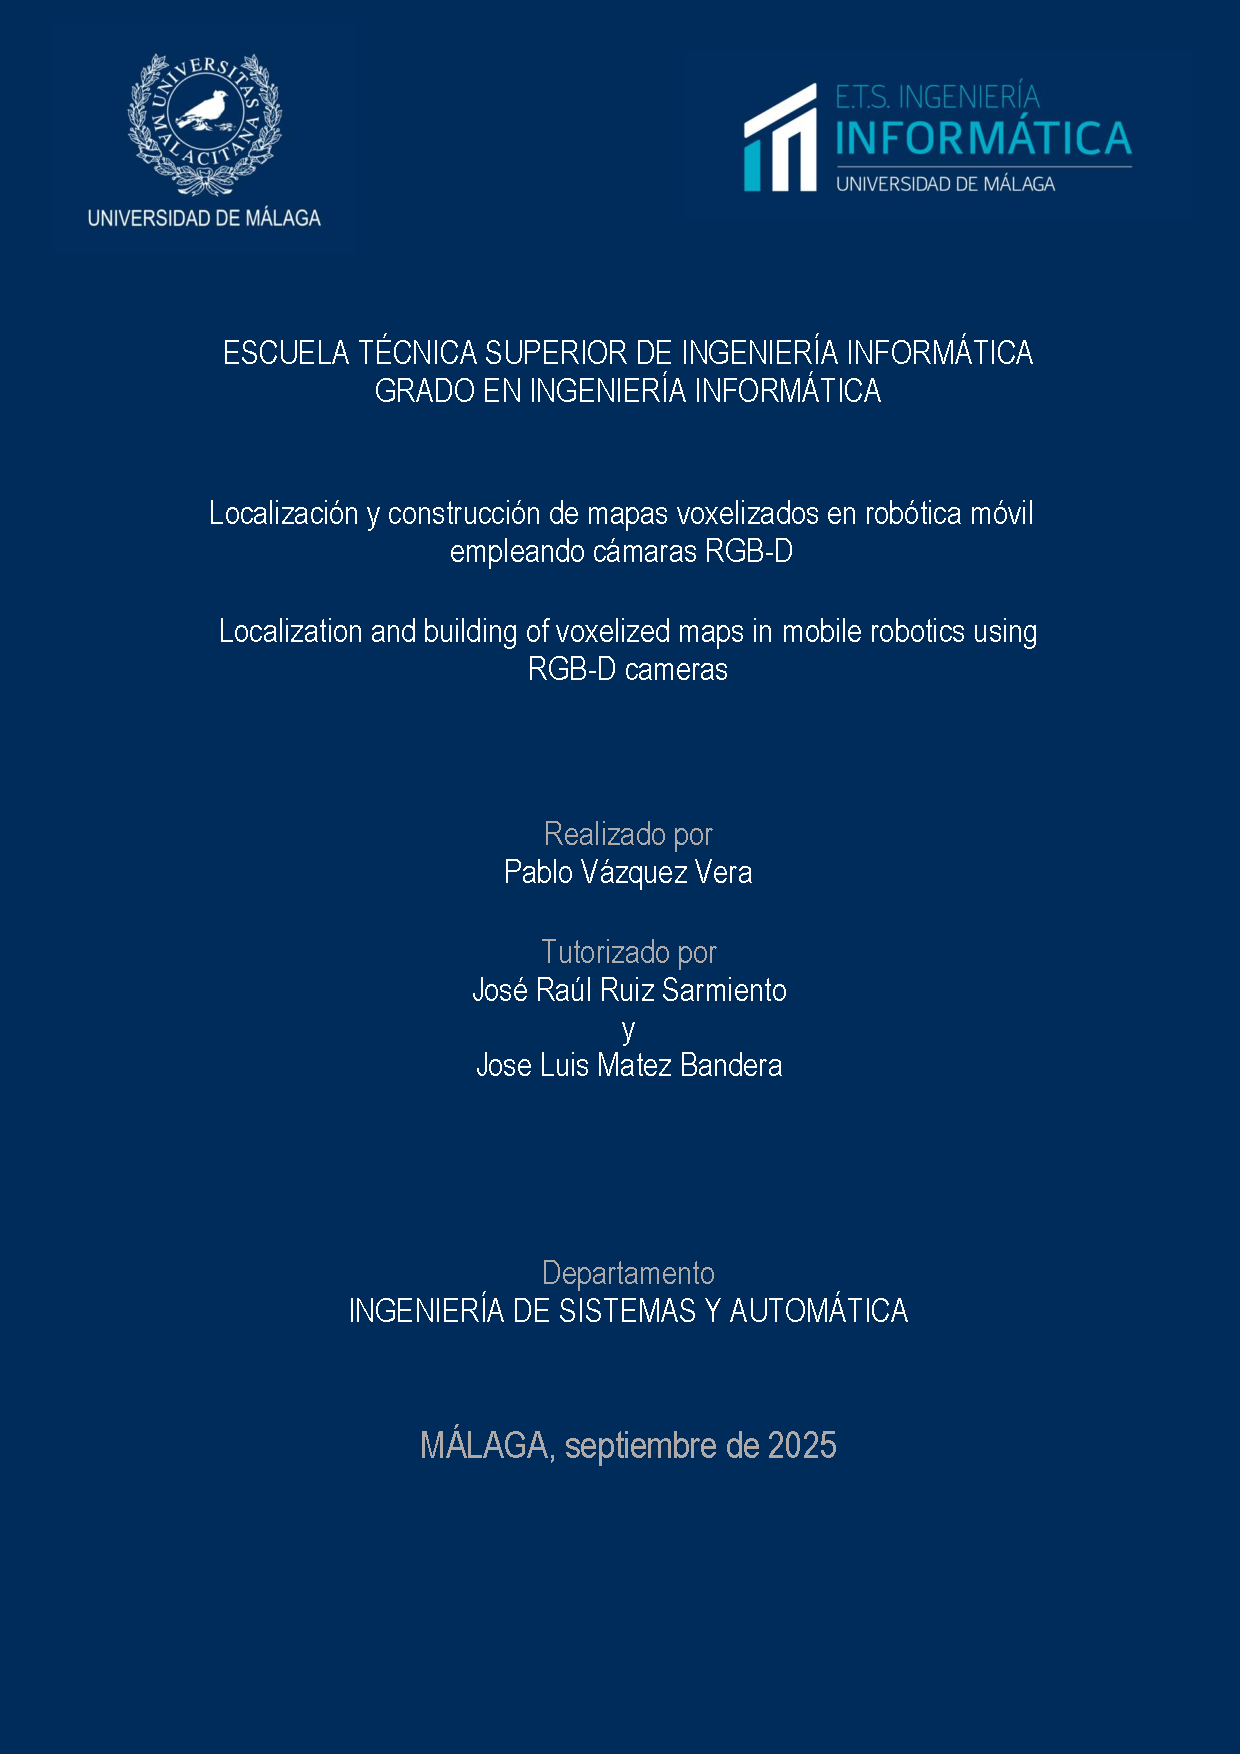
\includepdf[noautoscale=true, width=\paperwidth]{portada.pdf}

%% Abstract
\begin{abstract}
  Mobile robotics has profoundly transformed service robotics, expanding its possibilities and applications.
  By providing robots with autonomous mobility, it has become possible for them to move through complex environments without constant supervision.\newline
  Technologies such as computer vision, simultaneous localization and mapping (SLAM\cite{smith1987slam}), and advanced sensors enable these robots to avoid 
  obstacles and plan efficient routes. This has facilitated tasks such as cleaning, object transportation, and the delivery of food or 
  medicine in hospitals and hotels. Their implementation has reduced operating times and optimized resource utilization across multiple 
  industries.\newline
  In this context, the present work aims to investigate and analyze the feasibility of a mobile robotics project focused on the development 
  of a set of algorithms that can be used by robotic systems to autonomously localize themselves in an unknown environment while generating 
  a voxelized representation of it, commonly known as a map, using point clouds captured from the environment as the sole data source. 
  To accomplish this task, this project relies on the ROS2\cite{doi:10.1126/scirobotics.abm6074} development framework  as well as libraries specialized 
  in computer vision (Open3D\cite{Zhou2018}) and voxel map management (Bonxai\cite{faconti2024bonxai}). In addition, a set of metrics and 
  procedures will be proposed to validate the obtained results.\newline

  \bfseries{\large{Keywords:}}
  Mobile robotics, Voxel maps, Point clouds, Exploration of unknown environments.
\end{abstract}

\newpage

\renewcommand{\abstractname}{Resumen}

\begin{abstract}
  La robótica móvil ha transformado profundamente la robótica de servicio, ampliando sus posibilidades y aplicaciones.
  Al dotar a los robots de movilidad autónoma, se ha logrado que puedan desplazarse en entornos complejos sin supervisión constante.\newline
  Tecnologías como la visión por computadora, el mapeo simultáneo (SLAM\cite{smith1987slam}) y los sensores avanzados permiten que estos robots eviten 
  obstáculos y planifiquen rutas eficientes. Esto ha facilitado tareas de limpieza, transporte de objetos y entrega de alimentos o 
  medicinas en hospitales y hoteles. Su implementación ha reducido tiempos de operación y optimizado el uso de recursos en múltiples 
  industrias. \newline
  En este contexto, el presente documento tiene como objetivo investigar y analizar la viabilidad de un proyecto de robótica móvil, 
  centrado en el desarrollo de una serie de algoritmos que puedan ser usados por sistemas robóticos para localizarse de manera 
  autónoma en un entorno desconocido, a la vez que generan una representación voxelizada de este, comúnmente conocida como mapa, 
  recibiendo como única fuente de datos nubes de puntos capturadas del entorno. Para llevar a cabo esta tarea, este proyecto se apoya 
  en la plataforma de desarrollo ROS2\cite{doi:10.1126/scirobotics.abm6074} y librerías especializadas en la visión por computador (Open3D\cite{Zhou2018}) y la gestión de 
  mapas voxelizados (Bonxai\cite{faconti2024bonxai}). Además, se propondrán una serie de métricas y procedimientos para validar los resultados obtenidos.\newline

  \bfseries{\large{Palabras clave:}}
  Robótica móvil, Mapas voxelizados, Nubes de puntos, Exploración de entornos desconocidos.
\end{abstract}

\tableofcontents

%% Sections
\section{Introducción}

\subsection{Motivación}
La robótica es una disciplina que ha ampliado sus fronteras en los últimos años, y su aplicación ha demostrado ser 
increíblemente beneficiosa en una gran cantidad de materias, atrayendo la atención tanto de investigadores y profesionales de todo el 
mundo como de empresas e inversores interesados en su desarrollo y aplicación. \newline
Una de las ramas más prometedoras de la robótica es la robótica móvil, que se centra en el diseño y desarrollo de robots capaces 
de moverse de manera autónoma en entornos dinámicos. Esta rama es una de las más complejas y, a la vez, fascinantes, ya que implica 
la integración de diversas disciplinas como la inteligencia artificial, la visión por computadora y el control de sistemas, que 
deben trabajar en perfecta sintonía para lograr que el robot sea capaz de navegar y operar de manera eficiente en entornos que 
pueden ser impredecibles y cambiantes. \newline
La tarea que nos ocupa en este documento es el desarrollo de algoritmos que permitan a un sistema robótico localizarse en un entorno 
desconocido a la vez que genera una representación voxelizada de este, comúnmente conocida como mapa. Para llevar a cabo esta tarea, 
el robot recibirá como única fuente de datos nubes de puntos capturadas del entorno. Además, se calcularán una serie de métricas para 
validar la calidad de los resultados obtenidos en diferentes escenarios.\newline
Este proyecto plantea una serie de desafíos ligados a la naturaleza de los datos que se utilizan, ya que las nubes de puntos son 
representaciones tridimensionales del entorno que pueden ser:  
\begin{itemize}
  \item  \textbf{Computacionalmente costosas}: 
    Las nubes de puntos pueden contener millones de puntos, lo que requiere un procesamiento intensivo para extraer información útil.
  \item  \textbf{Ruidosas}:
    Las nubes de puntos pueden contener ruido debido a errores en la captura de datos intrínsecos a la naturaleza de los sensores.
  \item  \textbf{Incompletas}:
    Las nubes de puntos pueden no representar completamente el entorno debido a limitaciones en la cobertura del sensor o a 
    obstrucciones físicas en el entorno.
\end{itemize}
\begin{figure}[h]
  \centering
    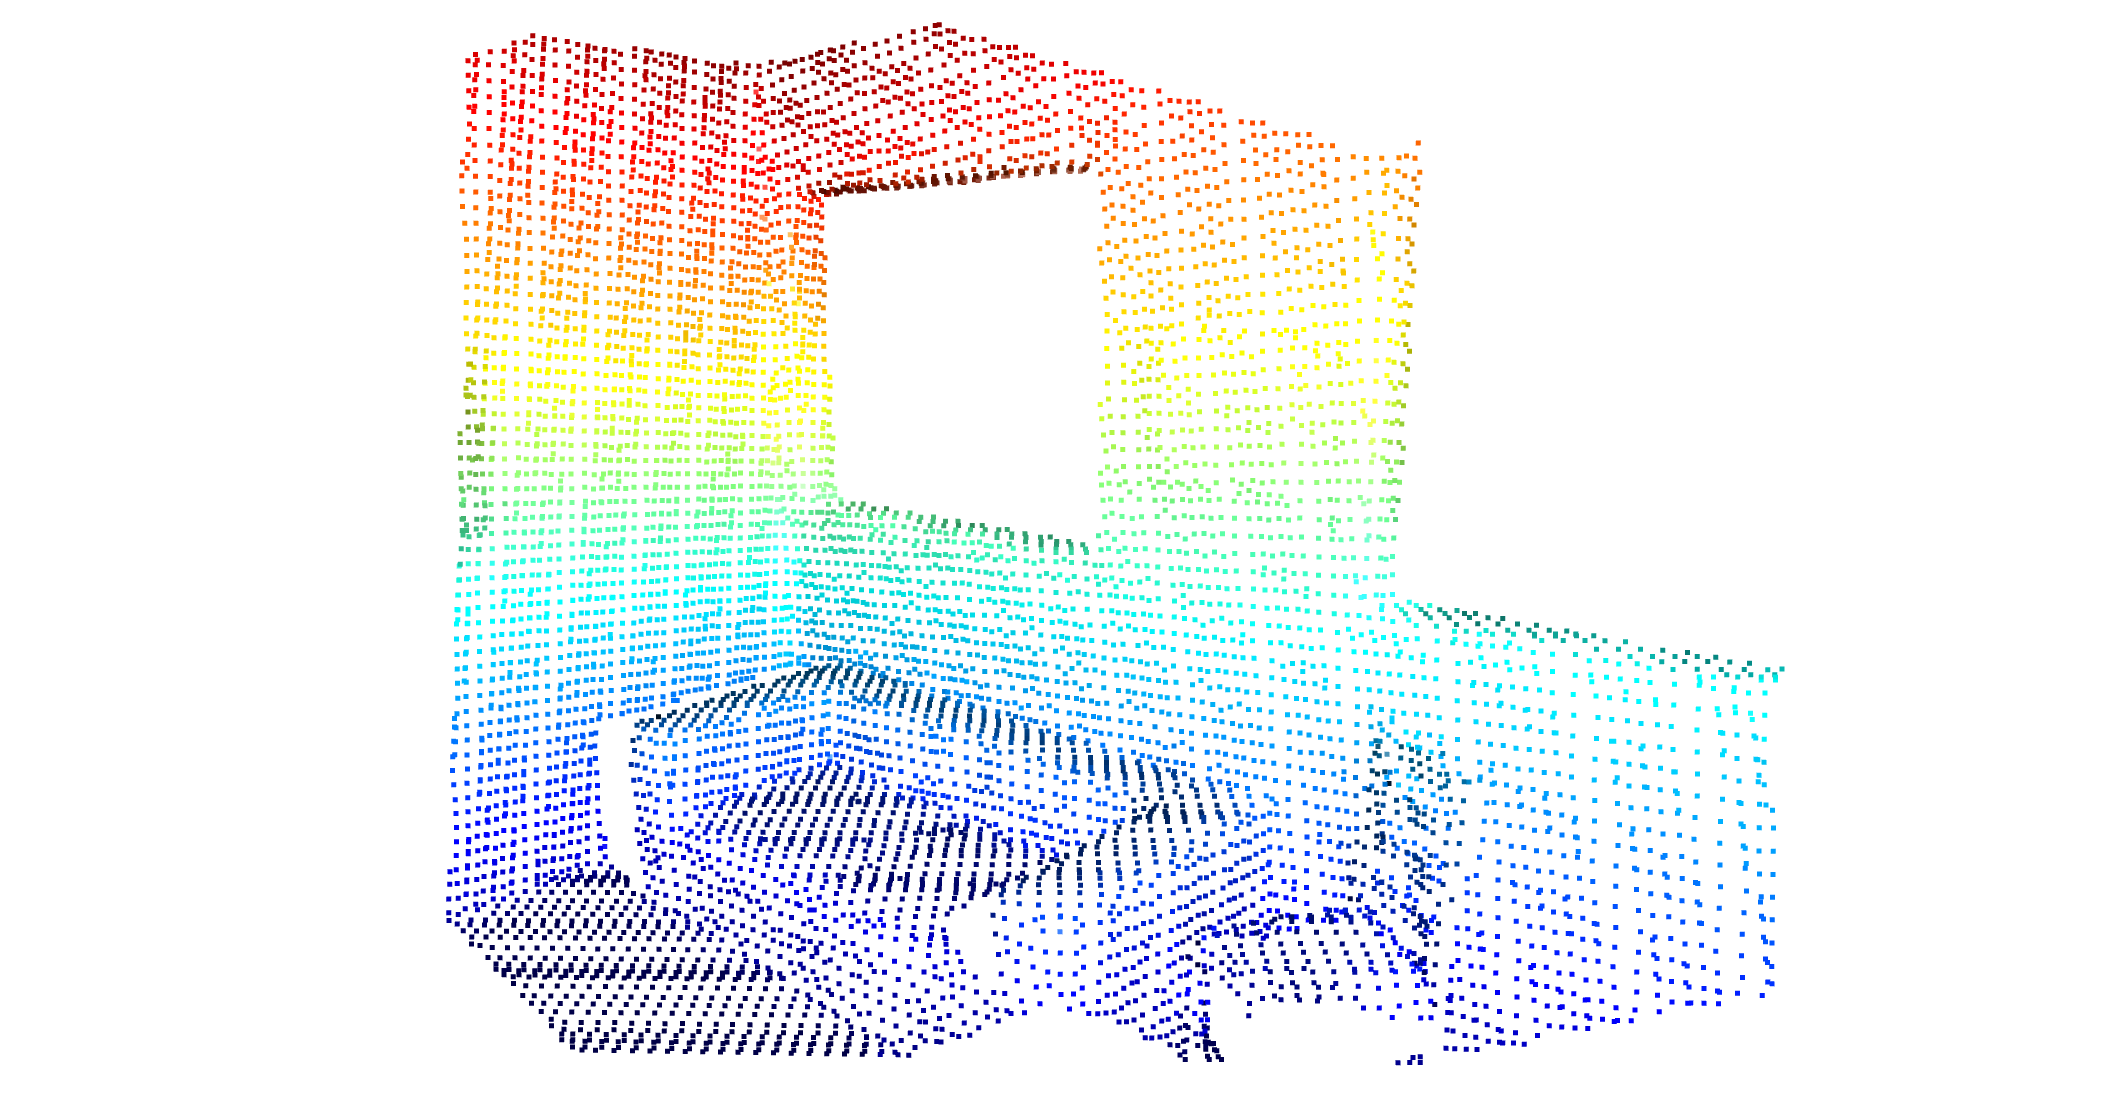
\includegraphics[width=0.5\textwidth]{Point_cloud_example.png}
  \caption{Imagen de una nube de puntos.}
\end{figure}
Esto nos llevará a explorar diversas técnicas de procesamiento de datos y algoritmos de localización y mapeo, así como a 
considerar las limitaciones y oportunidades que presenta el uso de nubes de puntos y los mapas voxelizados en la 
robótica móvil. \newline
Entre las herramientas y técnicas de interés más destacadas relacionadas con la casuística que se trata, se encuentra 
el uso de ICP (Iterative Closest Point de Open3D\cite{Zhou2018}) para la alineación de nubes de puntos y, por consiguiente, la 
obtención de la posición y orientación relativa del sistema respecto de pasos anteriores. Además, se ha seleccionado la librería 
Bonxai\cite{faconti2024bonxai} para la generación, manipulación y almacenamiento de mapas voxelizados, que permite gestionarlos de 
manera eficiente. También se hace uso de la amplia gama de herramientas y bibliotecas proporcionadas por ROS\cite{doi:10.1126/scirobotics.abm6074} 
en su segunda versión, ROS2\cite{doi:10.1126/scirobotics.abm6074}, para la implementación de los algoritmos de localización y mapeo, así como de la potencia y 
versatilidad de lenguajes de programación como Python\cite{python} y C++\cite{cpp} . \newline

\subsection{Objetivos}

El objetivo principal de este proyecto es desarrollar una serie de algoritmos que permitan a un sistema robótico localizarse en un 
entorno desconocido y generar un mapa voxelizado de este entorno utilizando nubes de puntos como única fuente de datos. 
Para lograr este objetivo, se ha de llevar a cabo una serie de tareas específicas:
\begin{itemize}
  \item \textbf{Diseño de un flujo de trabajo.} Para desarrollar este flujo de trabajo es necesario diseñar:
   \begin{itemize}
    \item \textbf{Sincronización de mensajes:} Se debe establecer un mecanismo de sincronización que permita 
      recibir y procesar las nubes de puntos de manera eficiente, asegurando que los datos estén disponibles en el momento 
      adecuado para su procesamiento. Además, se debe considerar cómo se gestionará la comunicación entre los diferentes 
      componentes del sistema, incluyendo la adquisición de datos, el procesamiento, la localización y la generación del mapa.
    \item \textbf{Preprocesamiento de los datos:} Se debe realizar un preprocesamiento de las nubes de puntos 
      para eliminar ruido y mejorar la calidad de los datos. Esto puede incluir técnicas como filtrado, segmentación y 
      reducción de ruido, así como la normalización de los datos para facilitar su procesamiento posterior.
    \item \textbf{Cálculo de la posición y orientación:} Se debe implementar un algoritmo que permita calcular la posición y orientación del 
      robot en el entorno a partir de las nubes de puntos recibidas. Esto puede incluir técnicas como ICP (Iterative Closest Point Open3D\cite{Zhou2018}) 
      para alinear las nubes de puntos y estimar la pose relativa del robot.
    \item \textbf{Construcción del mapa voxelizado:} Se debe utilizar alguna herramienta para la generación y manipulación 
      de mapas voxelizados, como Bonxai\cite{faconti2024bonxai}, para crear un mapa del entorno a partir de las nubes de puntos procesadas. 
      Esto puede incluir la creación de una estructura de datos eficiente para almacenar el mapa y la implementación de 
      algoritmos para actualizar el mapa a medida que se reciben nuevas nubes de puntos.
    \end{itemize}
  \item \textbf{Procedimiento de validación:} Es necesario estudiar y definir un procedimiento que permita evaluar de manera 
    objetiva la precisión y eficiencia del sistema de localización y mapeo desarrollado. Este procedimiento debe incluir:
    \begin{itemize}
    \item \textbf{Definición de métricas sobre la calidad de la localización:} Se deben definir métricas que permitan evaluar 
      la precisión de la localización del sistema en el entorno, considerando factores como la desviación respecto a la posición 
      real y la estabilidad de la localización a lo largo del tiempo.
    \item \textbf{Definición de métricas sobre la calidad del mapa:} Se deben definir métricas que permitan evaluar la calidad 
      del mapa generado por el sistema, considerando factores como la capacidad de representar adecuadamente el entorno.
    \end{itemize}
\end{itemize}

\subsection{Estructura del documento}

La estructura del documento se organiza en seis capítulos principales, cada uno de los cuales aborda un aspecto clave del proyecto:
\begin{itemize}
  \item \textbf{Capítulo 1: Introducción.} En este capítulo se presenta el contexto del proyecto, qué motiva el 
    desarrollo y la investigación llevada a cabo, así como se definen una serie de objetivos que se pretenden alcanzar.
  \item \textbf{Capítulo 2: Bases.} En este capítulo se proporciona una visión general de las bases teóricas y 
    técnicas que sustentan el proyecto, incluyendo conceptos clave como la localización y el mapeo.
  \item \textbf{Capítulo 3: Tecnologías usadas.} En este capítulo se describen las tecnologías y herramientas utilizadas 
    en el proyecto, incluyendo ROS2\cite{doi:10.1126/scirobotics.abm6074} y Bonxai\cite{faconti2024bonxai}, entre otros. 
    Además, se presentan las ventajas y desventajas de cada una de ellas, así como su aplicabilidad en el contexto del proyecto.
  \item \textbf{Capítulo 4: Localización y mapeo.} Este capítulo se centra en los algoritmos y técnicas utilizados para 
    la localización y el mapeo del sistema en un entorno desconocido, incluyendo la alineación de nubes de puntos y la generación 
    de mapas voxelizados.
  \item \textbf{Capítulo 5: Validación de resultados.} En este capítulo se presentan los resultados obtenidos en el proyecto, 
    incluyendo la evaluación de la precisión y eficiencia del sistema de localización y mapeo, así como una comparativa entre 
    los enfoques desarrollados.
  \item \textbf{Capítulo 6: Conclusiones.} En este capítulo se presentan las conclusiones del proyecto, incluyendo una reflexión 
    sobre los logros alcanzados, las lecciones aprendidas y las posibles direcciones futuras de investigación y desarrollo en el 
    campo de la robótica móvil.
\end{itemize}
\newpage

\section{Bases}

\subsection{Conceptos clave en robótica móvil}

En el contexto de la robótica móvil, los sensores que generan nubes de puntos —como LIDAR, cámaras RGB-D o sensores 
estereoscópicos— permiten obtener representaciones tridimensionales del entorno que son fundamentales para la localización 
y el mapeo. A partir de estas mediciones se definen diversas variables clave para describir el estado del robot y su relación con 
el entorno.

\begin{itemize}
  \item \textbf{Pose}: Variable central que describe la posición y orientación del robot en el espacio. En el caso bidimensional 
  se representa como:
  \[
  \mathbf{x} = [x, y, \theta]^{T}
  \]
  mientras que en 3D se extiende a:
  \[
  \mathbf{x} = [x, y, z, q_x, q_y, q_z, q_w]^{T}
  \]
  donde \( q_x, q_y, q_z, q_w \) corresponden a los cuaterniones que definen la orientación.
  \item \textbf{Traslación y rotación}: La traslación se refiere al desplazamiento del robot entre dos instantes de tiempo 
  consecutivos, estimado mediante el alineamiento de nubes de puntos (por ejemplo, usando algoritmos como ICP). Junto con la 
  traslación, se obtiene la rotación, que describe el cambio de orientación.
  \item \textbf{Drift}: Corresponde al error acumulado en la estimación de la pose debido al ruido sensorial, imprecisiones en 
  el alineamiento y propagación de errores de integración a lo largo del tiempo. La magnitud del drift determina la confiabilidad 
  de la trayectoria estimada y, en ausencia de cierre de bucle, tiende a crecer indefinidamente.
\end{itemize}
Otras variables relevantes derivadas de las nubes de puntos incluyen:
\begin{itemize}
    \item \textbf{Correspondencias}: Asociaciones entre puntos de la nube actual y del mapa previo.
    \item \textbf{Transformación estimada}: Matriz homogénea \( \mathbf{T} \in SE(3) \) que combina traslación y rotación para llevar la nube actual al marco de referencia global.
    \item \textbf{Error de registro}: Medida de la calidad del alineamiento de nubes, utilizada como criterio de convergencia en algoritmos iterativos.
\end{itemize}
El análisis de estas variables es crucial para el diseño de algoritmos de SLAM\cite{smith1987slam}, navegación autónoma y reconstrucción de entornos 
tridimensionales.

\subsection{Mapas voxelizados}

\subsubsection{Introducción a los mapas voxelizados}
La idea de los mapas voxelizados surgió como una extensión natural de los conceptos utilizados en la representación 
de imágenes digitales en dos dimensiones, aplicados al espacio tridimensional. Mientras que una imagen está compuesta 
por píxeles (elementos de imagen), un volumen tridimensional puede representarse mediante vóxeles (volumetric pixels), 
es decir, pequeñas celdas cúbicas que subdividen el espacio en una cuadrícula regular. \newline

\begin{figure}[h]
  \centering
    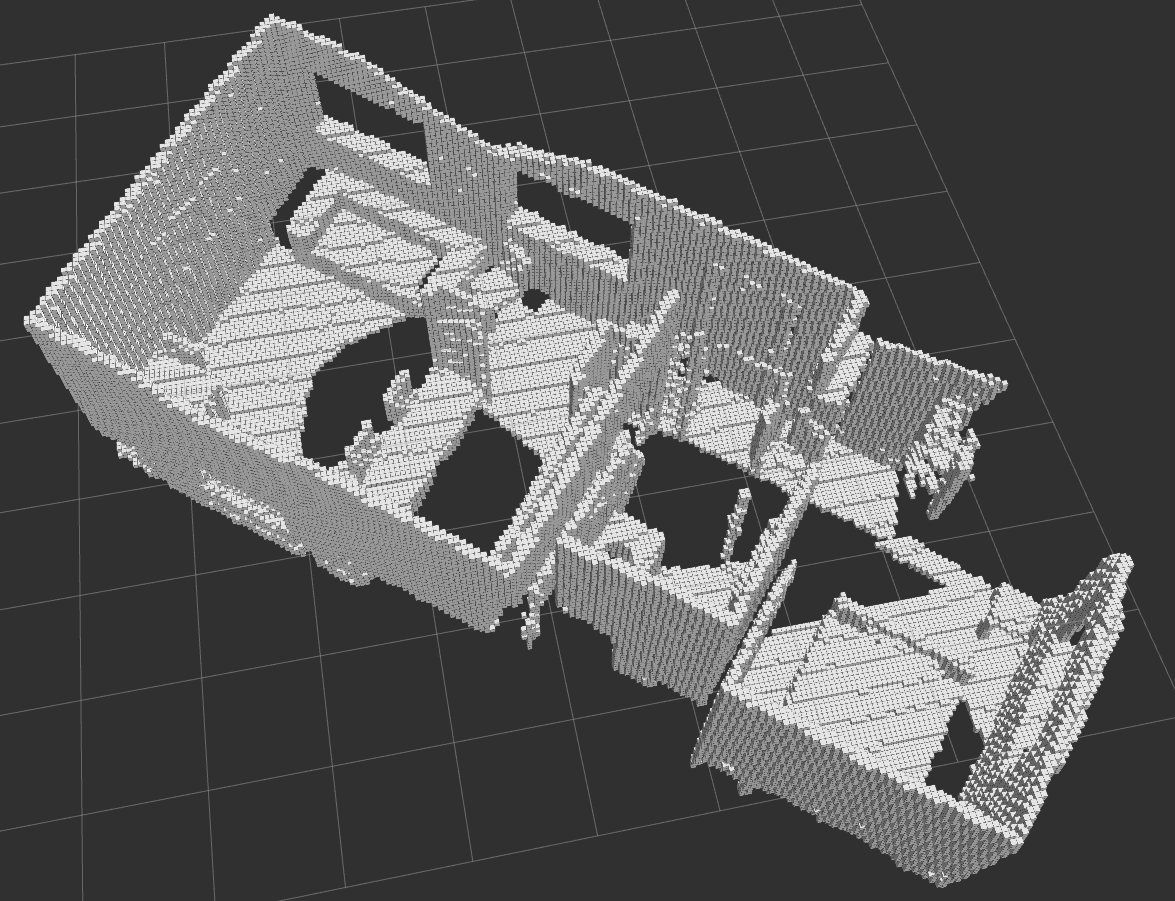
\includegraphics[width=0.5\textwidth]{Voxel_map_example.png}
  \caption{Imagen de un mapa voxelizado.}
\end{figure} 

El uso de vóxeles para modelar estructuras internas a partir de tomografías y resonancias comenzó en los años 70 y 80, 
cuando las capacidades computacionales posibilitaron el procesamiento volumétrico de datos médicos \cite{wired1996voxels_medical}. 
El proyecto pionero VOXEL-MAN en 1986 representó las primeras visualizaciones 3D voxelizadas, incluyendo la combinación de imágenes 
de CT y MRI \cite{voxelman1986history}. Un vóxel, equivalente tridimensional del píxel, ha sido definido como una unidad de valor en 
una rejilla 3D utilizada especialmente en visualización médica y científica \cite{wiki_voxel_definition}. Además, 
el algoritmo Marching Cubes de 1987 fue un hito en la extracción eficiente de superficies isosuperficiales desde datos 
voxelizados \cite{lorensen1987marchingcubes}. Estos desarrollos precedentes sentaron las bases para la adopción posterior 
de mapas voxelizados en robótica, navegación y planificación de movimiento.


\subsubsection{Características de los mapas voxelizados}

Un mapa voxelizado divide un espacio tridimensional en una cuadrícula regular de celdas cúbicas, denominadas voxeles 
(volumetric pixels). Cada voxel puede contener información binaria (ocupado/libre), probabilística (por ejemplo, con modelos 
bayesianos como los octomapas), o datos más complejos como intensidad, color o etiquetas semánticas. Entre sus características 
principales se destacan:

\begin{itemize}
  \item \textbf{Representación volumétrica discreta:} Los mapas voxelizados dividen el espacio tridimensional en una rejilla cúbica 
  regular compuesta por pequeñas celdas llamadas voxeles. Cada voxel representa una porción del espacio con una resolución 
  determinada, lo que permite una representación explícita del volumen y no solo de la superficie.
  \item \textbf{Resolución configurable:} La resolución del mapa puede ajustarse modificando el tamaño de los voxeles. Una 
  resolución más alta (voxeles más pequeños) proporciona mayor detalle, pero aumenta el consumo de memoria y el coste 
  computacional. Por el contrario, resoluciones más bajas reducen la precisión, pero permiten una operación más eficiente.
  \item \textbf{Estructura espacial regular:} La organización de los datos en una cuadrícula facilita la implementación de 
  algoritmos paralelos y el acceso constante a la información espacial, lo que es útil en cálculos de visibilidad, planificación 
  de trayectorias y simulaciones físicas.
  \item \textbf{Facilidad para representar ocupación:} Cada voxel puede almacenar un valor que indique si el espacio está ocupado, 
  libre o desconocido. Esta propiedad es fundamental para la planificación y la detección de colisiones en robótica y simulación.
  \item \textbf{Extensibilidad de la información por voxel:} Los voxeles pueden contener no solo información binaria (ocupado/libre), 
  sino también:
  \begin{itemize}
    \item \textbf{Probabilidades:} Representar la probabilidad de ocupación de un voxel, lo que permite manejar incertidumbres 
    en la percepción.
    \item \textbf{Intensidad o color:} Almacenar información adicional como la intensidad de la señal o el color asociado a cada voxel, 
    lo que es útil en aplicaciones de visión por computadora y reconstrucción 3D.
    \item \textbf{Etiquetas semánticas:} Asignar etiquetas a los voxeles para identificar objetos o características del entorno, 
    lo que es especialmente útil en aplicaciones de robótica móvil y percepción semántica.
    \item \textbf{Normales de superficie:} Almacenar información sobre la orientación de las superficies dentro de los voxeles, 
    lo que es útil para la reconstrucción de superficies y la simulación física.
    \end{itemize}
    \item \textbf{Compatibilidad con estructuras jerárquicas:} Para mejorar la eficiencia en almacenamiento y consultas, los mapas 
    voxelizados pueden implementarse con estructuras jerárquicas como los octrees, que dividen el espacio de forma adaptativa según 
    la densidad de información.
    \item \textbf{Eficiencia en consultas espaciales:} Gracias a su estructura regular (o jerárquica en el caso de octrees), 
    los mapas voxelizados permiten realizar operaciones como:
    \begin{itemize}
    \item \textbf{Búsqueda de vecinos:} Encontrar voxeles adyacentes de manera eficiente.
    \item \textbf{Intersección de rayos:} Determinar si un rayo intersecta con algún voxel, lo que es útil en 
    simulaciones de iluminación y trazado de rayos.
    \item \textbf{Colisiones:} Detectar colisiones entre objetos y el entorno representado por el mapa voxelizado, 
    lo que es esencial en robótica y simulación física.
    \end{itemize}
    \item \textbf{Idoneidad para entornos dinámicos:} La representación voxelizada puede actualizarse de forma local cuando se detectan 
    cambios en el entorno, lo que permite mantener mapas actualizados en tiempo real, aspecto esencial para aplicaciones robóticas y 
    vehículos autónomos.
  \end{itemize}

\subsubsection{Aplicaciones de los mapas voxelizados}
El uso de los mapas voxelizados se ha ampliado a diversos campos con el paso del tiempo gracias a las mejoras en computación, 
tecnologías de captura de datos e inversiones en investigación y desarrollo del área. Algunas de las aplicaciones más 
destacadas incluyen:

\begin{itemize}
  \item \textbf{Robótica móvil y navegación autónoma:} Los mapas voxelizados se utilizan para representar el entorno tridimensional 
  de un robot o vehículo autónomo. Se emplean para la planificación de trayectorias, detección de obstáculos y navegación segura.
  \begin{itemize}
    \item \textbf{Ventajas:} Permiten representar obstáculos a distintas alturas, útil en entornos no planos. Se integran bien con 
    sensores como LIDAR o cámaras RGB-D. Facilitan el ray tracing para simulaciones de sensores y planificación.
    \item \textbf{Inconvenientes:} Alta demanda de memoria y procesamiento, especialmente en espacios grandes. Requieren mecanismos 
    eficientes de actualización en entornos dinámicos.
  \end{itemize}
  \item \textbf{Reconstrucción 3D de escenas:} Los mapas voxelizados permiten reconstruir entornos tridimensionales desde datos de 
  sensores (escáneres láser, cámaras estereoscópicas, etc.).
  \begin{itemize}
    \item \textbf{Ventajas:} Buen manejo de ruido y fusión de múltiples vistas. Permiten interpolar datos faltantes o parciales 
    de forma robusta.
    \item \textbf{Inconvenientes:} La densidad del modelo puede hacer que sea difícil de almacenar o transmitir. Generalmente 
    se requiere un posprocesamiento para renderizado o análisis.
  \end{itemize}
  \item \textbf{Medicina e imagen biomédica:} Se usan para modelar órganos y tejidos en 3D, a partir de escaneos como tomografía 
  (CT) o resonancia magnética (MRI), permitiendo diagnósticos y planificación quirúrgica.
  \begin{itemize}
    \item \textbf{Ventajas:} Representan estructuras internas de forma precisa y continua. Permiten segmentación automática 
    y simulaciones médicas.
    \item \textbf{Inconvenientes:} Altos requisitos computacionales para procesar volúmenes detallados. Requieren software 
    especializado para su interpretación.
  \end{itemize}
  \item \textbf{Simulación física y entornos virtuales:} Se utilizan en motores de física y simulación para modelar el 
  comportamiento de materiales, fluidos o entornos destructibles.
  \begin{itemize}
    \item \textbf{Ventajas:} Representación volumétrica adecuada para materiales no rígidos o granularidad. Permiten simulaciones 
    dinámicas y realistas de colisiones o fluidos.
    \item \textbf{Inconvenientes:} Las simulaciones físicas con vóxeles pueden ser computacionalmente más intensas que con mallas.
  \end{itemize}
  \item \textbf{Videojuegos y gráficos por computadora:} Se usan para construir mundos destructibles o interactivos, como en 
  juegos con estética voxel (por ejemplo, Minecraft).
  \begin{itemize}
    \item \textbf{Ventajas:} Simplicidad para modelar entornos que cambian o se destruyen. Representación directa en memoria 
    de entornos interactivos.
    \item \textbf{Inconvenientes:} Apariencia visual menos realista comparada con modelos basados en polígonos. No adecuados 
    para gráficos de alta fidelidad sin posprocesado.
  \end{itemize}
  \item \textbf{Exploración subterránea y minería:} Los mapas voxelizados se utilizan para representar túneles, cavidades o 
  cuerpos geológicos, permitiendo el análisis y la planificación de rutas de extracción.
  \begin{itemize}
    \item \textbf{Ventajas:} Manejan entornos 3D complejos con estructuras irregulares. Permiten planificación segura en 
    zonas de difícil acceso.
    \item \textbf{Inconvenientes:} Requiere integrar datos de múltiples fuentes con resolución variable. La visualización y 
    el análisis pueden ser más complejos que con mapas 2D.
  \end{itemize}
\end{itemize}

\section{Tecnologías usadas}
Esta sección se centra en introducir las tecnologías usadas para el proceso completo de desarrollo del proyecto. 
Se introducen los lenguajes de programación utilizados, las plataformas de desarrollo, librerías externas y frameworks usados
a lo largo del proyecto.

\subsection{Lenguajes}
En el desarrollo del proyecto se han utilizado varios lenguajes para abordar diferentes aspectos del sistema.
Entre ellos se encuentran:

\begin{itemize}
  \item \textbf{Python:\cite{python}} Python\cite{python} es un lenguaje de programación interpretado, de alto nivel y con una sintaxis clara y legible. 
  Fue diseñado para ser fácil de aprender y usar, lo que lo hace ideal tanto para principiantes como para desarrolladores 
  avanzados. Es multiparadigma (soporta programación orientada a objetos, funcional e imperativa) y tiene una gran cantidad 
  de bibliotecas disponibles. La integración de Python\cite{python} en ROS2\cite{doi:10.1126/scirobotics.abm6074} permite el desarrollo rápido de prototipos y la implementación
  de algoritmos complejos de procesamiento de datos, control y comunicación entre nodos. Python\cite{python} es el lenguaje principal
  de este proyecto, usado para la implementación de nodos de ROS2\cite{doi:10.1126/scirobotics.abm6074}, control del flujo de datos, la lógica para el cálculo 
  de la pose, métricas de validación y manipulación de nubes de puntos.
  \begin{figure}[h]
    \centering
      
\includegraphics[width=0.5\textwidth]{Python_logo.png} 
    \caption{Logo de Python\cite{python}.}
  \end{figure} 
  \item \textbf{C++:\cite{cpp}} Lenguaje de programación compilado, de propósito general, conocido por su alto rendimiento, 
  control sobre el hardware y capacidades de programación orientada a objetos. Es ampliamente utilizado en sistemas embebidos, 
  videojuegos y especialmente en aplicaciones donde el rendimiento y la eficiencia son críticos. La integración de C++\cite{cpp} 
  en ROS2\cite{doi:10.1126/scirobotics.abm6074} permite el desarrollo de nodos de alto rendimiento, especialmente aquellos que requieren procesamiento intensivo
  de datos o interacción directa con hardware. En este proyecto, C++\cite{cpp}  se utiliza para nodos de almacenamiento y gestión del
  mapa voxelizado e interacción con la librería Bonxai\cite{faconti2024bonxai}, que proporciona una interfaz eficiente para la manipulación de mapas
  voxelizados.
  \begin{figure}[h]
    \centering
      
\includegraphics[width=0.2\textwidth]{C++_logo.png}
    \caption{Logo de C++\cite{cpp} .}
  \end{figure} 
  \item \textbf{XML:\cite{xml}} XML\cite{xml} (eXtensible Markup Language) es un lenguaje de marcado diseñado para almacenar y 
  transportar datos de forma estructurada y legible tanto para humanos como para máquinas. En ROS2\cite{doi:10.1126/scirobotics.abm6074}, XML\cite{xml} se utiliza principalmente 
  en la configuración y descripción de componentes del sistema robótico debido al sistema de descripciones de robots URDF y 
  XACRO, su legibilidad, interoperabilidad y amplia adopción en la industria. En este proyecto, XML\cite{xml} se utiliza para
  definir la configuración de los nodos de ROS2\cite{doi:10.1126/scirobotics.abm6074}, incluyendo parámetros, tópicos y dependencias entre servicios.
  \begin{figure}[h]
    \centering
      
\includegraphics[width=0.5\textwidth]{xml_logo.png}
    \caption{Logo de XML\cite{xml}.}
  \end{figure} 
  \item \textbf{YAML:\cite{yaml}} YAML\cite{yaml} (Yet Another Markup Language, o más correctamente YAML\cite{yaml} Ain't Markup Language) es un formato de 
  serialización de datos basado en texto, muy usado para representar información de forma estructurada y legible por humanos.
  Sus principales usos son como formato de configuración y para el intercambio de datos entre aplicaciones. En ROS2\cite{doi:10.1126/scirobotics.abm6074}, YAML\cite{yaml} se 
  utiliza para definir parámetros de nodos, configuraciones de lanzamiento y otros aspectos del sistema robótico. En este proyecto, 
  YAML\cite{yaml} se utiliza para almacenar configuraciones de nodos, parámetros de algoritmos y otros datos estructurados necesarios para 
  la ejecución del sistema.
  \begin{figure}[h]
    \centering
      
\includegraphics[width=0.2\textwidth]{yaml_logo.png}
    \caption{Logo de YAML\cite{yaml}.}
  \end{figure} 
  \item \textbf{CMAKE:\cite{cmake}} CMake\cite{cmake} es un lenguaje de configuración y scripting especializado para la construcción de software.
  Se usa como herramienta de automatización de compilación que utiliza archivos llamados CMakeLists.txt para describir 
  cómo debe compilarse y enlazarse un proyecto de software. CMake\cite{cmake} es usado en ROS2\cite{doi:10.1126/scirobotics.abm6074} debido a que es la herramienta 
  estándar para la construcción de paquetes y nodos, facilitando la gestión de dependencias, la configuración del entorno
  de compilación y la generación de archivos de configuración necesarios para la ejecución de los nodos desarrollados en C++\cite{cpp} .
  \begin{figure}[h]
    \centering
      
\includegraphics[width=0.2\textwidth]{cmake_logo.png}
    \caption{Logo de CMake\cite{cmake}.}
  \end{figure} 
  \item \textbf{LaTeX:\cite{lamport1994latex}} LaTeX\cite{lamport1994latex} es un sistema de composición de documentos basado en el lenguaje de tipografía TeX. Está 
  diseñado para la creación de documentos de alta calidad tipográfica, especialmente aquellos que incluyen fórmulas matemáticas 
  complejas, referencias cruzadas, bibliografías y estructuras organizadas como capítulos, secciones y tablas.
  \begin{figure}[h]
    \centering
      
\includegraphics[width=0.2\textwidth]{Latex_logo.png}
    \caption{Logo de LaTeX\cite{lamport1994latex}.}
  \end{figure} 
\end{itemize}

\subsection{Entorno, software y herramientas de desarrollo}
  En el desarrollo del proyecto se han utilizado varias herramientas y entornos para facilitar la implementación, el desarrollo
  y la prueba del código. Entre ellos se encuentran:
  \begin{itemize}
    \item
      \textbf{ROS2\cite{doi:10.1126/scirobotics.abm6074} (Humble Hawksbill):} ROS 2 (Robot Operating System 2) es un marco de desarrollo y un conjunto de herramientas 
      diseñadas para facilitar la creación de sistemas robóticos complejos, modulares y distribuidos. Aunque su nombre sugiere que es 
      un sistema operativo, en realidad ROS 2 no es un sistema operativo tradicional, sino una capa de software que proporciona 
      abstracciones y servicios esenciales para el desarrollo de robots, como:
      \begin{itemize}
        \item \textbf{Comunicación entre componentes:} ROS 2 organiza el software robótico en nodos independientes que se comunican 
        entre sí usando tópicos, servicios y acciones. Esto permite una arquitectura modular y escalable.
        \item \textbf{Gestión de hardware:} ROS 2 interactúa con sensores y actuadores a través de drivers y interfaces de hardware.
        \item \textbf{Control en tiempo real:} ROS 2 está diseñado para trabajar con sistemas en tiempo real, permitiendo ejecutar 
        controladores que responden de manera precisa y rápida. 
        \item \textbf{Simulación, visualización y depuración:} ROS 2 se integra con herramientas como:
        \begin{itemize}
        \item \textbf{RViz:} Una herramienta de visualización que permite ver datos de sensores, mapas y estados del robot en 
        tiempo real.
        \item \textbf{ROS2\cite{doi:10.1126/scirobotics.abm6074} bag:} Un sistema de registro que permite grabar y reproducir datos de sensores y mensajes de ROS 2, 
        facilitando la depuración y el análisis de datos.
        \item \textbf{ROS2\cite{doi:10.1126/scirobotics.abm6074} doctor, trace, topic, etc.:} Herramientas de diagnóstico y monitoreo que permiten analizar el estado 
        del sistema, rastrear mensajes y verificar la comunicación entre nodos.
        \end{itemize} 
      \end{itemize}
      \begin{figure}[h]
        \centering
          
\includegraphics[width=0.2\textwidth]{Ros2_humble.png} 
        \caption{Logo de Ros2\cite{doi:10.1126/scirobotics.abm6074}.}
      \end{figure} 
      ROS 2 (Robot Operating System 2) es la evolución del sistema operativo para robots originalmente conocido como ROS 1. Fue 
      diseñado desde cero para resolver las limitaciones arquitectónicas y técnicas de ROS 1, ofreciendo una plataforma más robusta, 
      segura, flexible y adecuada para aplicaciones comerciales, industriales y en tiempo real. Estas mejoras vienen dadas por el uso de:
      \begin{itemize}
        \item \textbf{DDS (Data Distribution Service):} Un middleware de comunicación en tiempo real que permite la interoperabilidad 
        entre nodos, mejorando la escalabilidad, fiabilidad y seguridad de la comunicación.
        \item \textbf{RTOS (Real-Time Operating System):} Permite ejecutar nodos en sistemas operativos de tiempo real.
        \item \textbf{Soporte para múltiples lenguajes y plataformas:} ROS 2 ofrece soporte nativo para varios lenguajes de programación,
        como C++, Python y Rust, y es compatible con una amplia gama de sistemas operativos, incluyendo Linux, Windows y macOS.
        \item \textbf{Mejoras en el sistema de construcción:} Se usa colcon en lugar de catkin, lo que permite una construcción
        más eficiente y flexible de los paquetes de ROS 2.
      \end{itemize} 
      \item \textbf{Ubuntu\cite{ubuntu} (22.04 LTS):} Ubuntu\cite{ubuntu} es una distribución del sistema operativo Linux, basada en Debian, desarrollada por 
      Canonical. Es conocida por ser gratuita, de código abierto, estable y fácil de usar, tanto para usuarios nuevos como para 
      desarrolladores. En concreto, la versión 22.04 LTS (Long Term Support) es una versión de soporte a largo plazo,
      lo que significa que recibirá actualizaciones de seguridad y mantenimiento durante un período prolongado (5 años).
      Además de esto, se ha elegido esta versión en concreto por el soporte oficial de ROS 2 en la distribución Humble Hawksbill,
      su alta compatibilidad con las herramientas de desarrollo usadas, la fácil gestión de dependencias y el amplio uso 
      por parte de la comunidad de robótica.  \begin{figure}[h]
        \centering
          
\includegraphics[width=0.3\textwidth]{Ubuntu_logo.jpg} 
        \caption{Logo de Ubuntu\cite{ubuntu}.}
      \end{figure} 
      \item \textbf{Visual Studio Code\cite{vscode}:} Visual Studio Code\cite{vscode} es un editor de código fuente ligero y multiplataforma, desarrollado 
      por Microsoft. Es gratuito, de código abierto y compatible con una gran variedad de lenguajes de programación como C++\cite{cpp} , 
      Python\cite{python}, XML\cite{xml}, CMake\cite{cmake}, entre otros. Ofrece extensiones, depuración integrada, control de versiones (Git) y una interfaz 
      altamente personalizable. Se ha elegido usar este editor por su compatibilidad con los múltiples lenguajes usados en el 
      proyecto, su ligereza y rapidez, su amplia gama de extensiones y su integración con herramientas de desarrollo como CMake\cite{cmake} y ROS2\cite{doi:10.1126/scirobotics.abm6074}.
      \begin{figure}[h]
        \centering
          
\includegraphics[width=0.3\textwidth]{Vs_code_logo.png} 
        \caption{Logo de Visual Studio Code.}
      \end{figure} 
      \newpage
      \item \textbf{GitHub\cite{github}:} GitHub\cite{github} es una plataforma en línea para almacenar, compartir y colaborar en proyectos de software utilizando 
      el sistema de control de versiones Git. Permite a desarrolladores trabajar en proyectos, rastrear cambios en el código, 
      revisar contribuciones y gestionar versiones del software, todo desde un entorno centralizado basado en la web.
      \begin{figure}[h]
        \centering
          
\includegraphics[width=0.2\textwidth]{Github_logo.png} 
        \caption{Logo de GitHub\cite{github}.}
      \end{figure} 
      \item \textbf{Jupyter Notebook\cite{jupyter}:} Jupyter Notebook\cite{jupyter} es una herramienta interactiva que permite escribir y ejecutar código 
      en fragmentos llamados celdas. Aunque originalmente fue diseñado para usarse en un navegador web, también se puede utilizar 
      directamente desde entornos como Visual Studio Code (VS Code). Aunque está orientado a Python\cite{python}, también puede usarse con otros 
      lenguajes. La principal ventaja de Jupyter Notebook\cite{jupyter} es su capacidad para combinar código, texto, visualizaciones y otros elementos
      multimedia en un solo documento, lo que facilita la creación de informes interactivos y la documentación de proyectos. 
      En este proyecto se ha utilizado para documentar el proceso de análisis de resultados y la validación de los algoritmos implementados.  \begin{figure}[h]
        \centering
          
\includegraphics[width=0.2\textwidth]{Jupyter_logo.png} 
        \caption{Logo de Jupyter Notebook\cite{jupyter}.}
      \end{figure} 
      \newpage
      \item \textbf{Terminator\cite{terminator}:} Terminator\cite{terminator} es un emulador de terminal para sistemas operativos basados en Unix, que permite dividir la
      ventana de la terminal en múltiples paneles, facilitando la ejecución de varios comandos y la visualización de salidas
      simultáneamente. Es especialmente útil para desarrolladores y administradores de sistemas que necesitan trabajar
      con múltiples sesiones de terminal al mismo tiempo. En este proyecto, se ha utilizado para ejecutar y monitorear múltiples 
      nodos de ROS2\cite{doi:10.1126/scirobotics.abm6074} simultáneamente, facilitando la depuración y el control del flujo de datos entre los diferentes componentes del sistema.
      \begin{figure}[h]
        \centering
          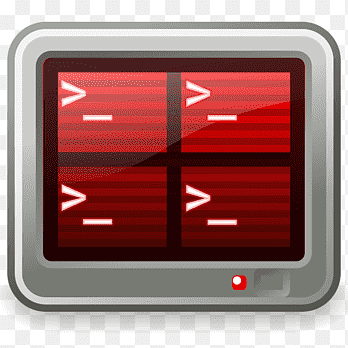
\includegraphics[width=0.2\textwidth]{Terminator.png} 
        \caption{Logo de Terminator\cite{terminator}.}
      \end{figure} 
\end{itemize}

\section{Flujo de trabajo para la Localización y Mapeo Simultaneo}

En esta sección primero se describen las funciones y componentes clave que entran en juego en el proceso. Posteriormente, se describirá 
el flujo de datos y la interacción entre los diferentes componentes del sistema y, por tanto, el flujo de trabajo 
completo de la aplicación.

\subsection{Conceptos, componentes y funciones clave}
En esta sección se detallan cada uno de los componentes clave que entran en juego en el flujo de trabajo del sistema, su base,
las funciones que desempeñan, los conceptos que lo sustentan y los detalles de su implementación.

\subsubsection{Gestión y sincronización de mensajes}
La gestión y sincronización de mensajes es un aspecto crucial en sistemas robóticos distribuidos, donde múltiples nodos trabajan de forma 
conjunta para lograr tareas complejas. En el contexto de ROS2\cite{doi:10.1126/scirobotics.abm6074}, los nodos se comunican entre sí mediante el intercambio de mensajes a
través de tópicos, servicios y acciones. La sincronización adecuada de estos mensajes es esencial para garantizar que los datos se procesen 
en el orden correcto y que las operaciones dependientes de múltiples fuentes se realicen de manera coherente. \newline
Para lograr una gestión y sincronización correcta de los mensajes para este proyecto y dado que la fuente de datos está almacenada en un 
archivo de tipo \textit{rosbag}, que es un tipo de archivo dedicado al almacenamiento de comunicaciones en ROS2\cite{doi:10.1126/scirobotics.abm6074}, 
se ha optado por el desarrollo de un nodo que se encargue de reproducir los mensajes adecuados en función de la disponibilidad de los principales nodos de procesamiento.\newline
Este nodo, llamado ''input\textunderscore data\textunderscore node'', se encarga de crear una estructura de datos que almacena los mensajes contenidos 
en el archivo \textit{rosbag} (grabación con los datos), ya que estos vienen serializados. Una vez leído este archivo y creada esta estructura de datos con los 
datos serializados, se irán leyendo los mensajes de forma ordenada, deserializando, formateando según el tipo de datos al que corresponda el mensaje 
y publicándolos en los tópicos correspondientes.

\paragraph{Conceptos clave:}
Los conceptos clave que sustentan este nodo son:
\begin{itemize}
  \item \textbf{Archivos \textit{rosbag}}: Un \textit{rosbag} es un archivo usado en ROS2\cite{doi:10.1126/scirobotics.abm6074} para registrar y reproducir datos de tópicos. Los 
  archivos \textit{rosbag} se almacenan en formato binario, guardando la secuencia de mensajes ROS capturados. Estos mensajes incluyen cabeceras, marcas de tiempo 
  y datos serializados. En nuestro caso, usaremos un archivo de este tipo para leer una grabación realizada previamente sobre un entorno simulado que 
  intentaremos recrear usando nuestro proceso de localización y mapeo.
  \item \textbf{Serialización y deserialización de mensajes}: La serialización es el proceso de convertir un objeto o estructura de datos en una secuencia 
  de bytes para su almacenamiento, y la deserialización es el proceso inverso, es decir, convertir una secuencia de bytes en un objeto o estructura de datos. 
  En ROS2\cite{doi:10.1126/scirobotics.abm6074}, los mensajes se serializan para su transmisión a través de la red o su almacenamiento en archivos \textit{rosbag}. En nuestro caso, los mensajes leídos del 
  archivo \textit{rosbag} vienen serializados, por lo que es necesario deserializarlos antes de poder usarlos. Esta acción será clave una vez leído el archivo \textit{rosbag} 
  y antes de publicar los mensajes en los tópicos correspondientes.
  \item \textbf{Publicación y suscripción a tópicos}: En ROS2\cite{doi:10.1126/scirobotics.abm6074}, los nodos pueden publicar mensajes en tópicos y suscribirse a ellos para recibir mensajes.
  La publicación y suscripción a tópicos es un mecanismo de comunicación fundamental en ROS2\cite{doi:10.1126/scirobotics.abm6074}, que permite la comunicación asíncrona entre nodos. En nuestro caso, 
  el nodo ''input\textunderscore data\textunderscore node'' publicará los mensajes deserializados en el tópico ''clean\textunderscore pcl'' para los datos que 
  correspondan a las nubes de puntos que se usarán para el proceso de mapeo y localización, y en el tópico ''clean\textunderscore pose'' para los datos que correspondan 
  a la pose original del robot, que se usará para aislar la pose real desde donde se capturaron las nubes de puntos y poder sacar métricas de precisión respecto a 
  esta pose.  
\end{itemize}

\paragraph{Funcionamiento del componente:}
Tal y como se ha descrito, el nodo ''input\textunderscore data\textunderscore node'' se encargará de leer el archivo \textit{rosbag}, deserializar los mensajes y
publicarlos en los tópicos correspondientes. El flujo de trabajo del nodo se puede describir de la siguiente manera:
\begin{itemize}
  \item \textbf{Inicialización}: La inicialización de este nodo está conformada por los siguientes pasos:
  \begin{itemize}
    \item \textbf{Inicialización de publicadores y suscriptores}: Al instanciar el nodo, se inicia la escucha y se prepara para la recepción de mensajes de los 
    siguientes tópicos:
    \begin{itemize}
      \item \textbf{Publicación de ''clean\textunderscore pose''}: Este servicio de publicación se encargará de enviar mensajes de tipo ''PoseStamped'' que 
      contienen la pose original desde la que se capturó el mensaje.
      \item \textbf{Publicación de ''clean\textunderscore pcl''}: Este servicio de publicación se encargará de enviar mensajes de tipo ''PointCloud2'' que 
      contienen la nube de puntos original.
      \item \textbf{Suscripción a ''new\textunderscore pose''}: Este suscriptor recibirá mensajes de tipo ''PoseStamped'' conteniendo la nueva pose calculada en función 
      del cálculo realizado por el servicio de publicación.
    \end{itemize}
    \item \textbf{Inicialización de lectura del archivo \textit{rosbag}}: Es necesario inicializar el sistema de lectura del archivo \textit{rosbag} para que se pueda iterar fácilmente
    a través de los mensajes que este contiene.
    \item \textbf{Inicialización de variables auxiliares para la ejecución}: Es necesario inicializar algunas variables auxiliares como índices, entre otras,  
    para la correcta ejecución del nodo.
  \end{itemize}
  \item \textbf{Respuestas provocadas por la recepción de mensajes a través del tópico ''new\textunderscore pose''}: Cada vez que se recibe un mensaje a través del tópico 
  ''new\textunderscore pose'' se inicia un proceso de respuesta que involucra los siguientes pasos:
  \begin{itemize}
    \item \textbf{Obtención de la última pose antes de la publicación de la nube de puntos}: Se leerá el archivo \textit{rosbag} almacenando siempre el último mensaje con etiqueta 
    ''gt\textunderscore odom'' de forma que, cuando se encuentre un mensaje conteniendo la nueva nube de puntos, se pueda deserializar y rellenar un mensaje de tipo ''PoseStamped'' 
    que contendrá la última pose asociada a este mensaje por el tópico ''clean\textunderscore pose''.
    \item \textbf{Obtención de las nubes de puntos}: Se continuará la lectura de los mensajes del archivo \textit{rosbag} hasta que se encuentre uno con la etiqueta 
    ''cloud\textunderscore in''. Entonces, se deserializarán los datos del mensaje y se rellenarán aquellos campos necesarios para publicar un mensaje de tipo ''PointCloud2''.
    Una vez se obtiene este mensaje de tipo ''PointCloud2'' relleno, este se publicará a través del tópico ''clean\textunderscore pcl'' junto con la pose asociada por el tópico 
    correspondiente.
  \end{itemize}
\end{itemize}
\begin{figure}[h]
  \centering
    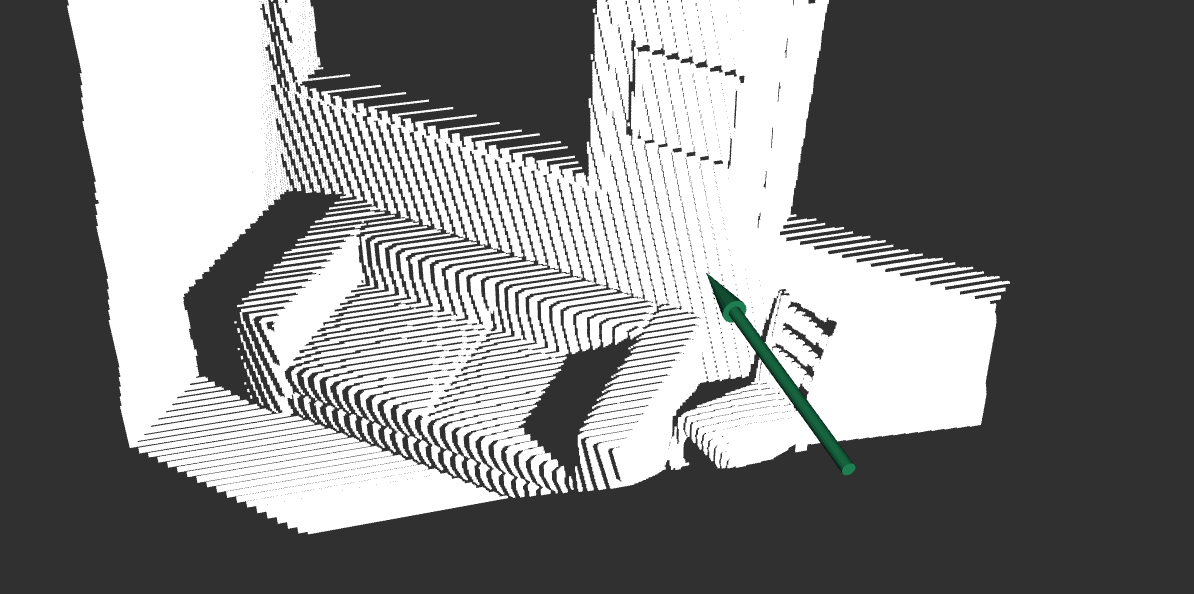
\includegraphics[width=0.7\textwidth]{rosbag_output.png}
  \caption{Imagen de una nube de puntos y pose asociada extraídas por el nodo ''input\textunderscore data\textunderscore node''.}
\end{figure}
En resumen, este nodo se encarga de iniciar el flujo de datos de entrada publicando los mensajes asociados con las nubes de puntos y la pose asociada. Una vez se ha iniciado
este flujo, continuará publicando estos mensajes cada vez que reciba un mensaje por parte del nodo de localización (determinando así que este está listo para recibir otro),
y así hasta que se complete la lectura.

\subsubsection{Adición de ruido a los datos originales}
Comprobar la resiliencia de nuestro flujo de trabajo frente al ruido es una parte esencial de este estudio, ya que acerca la simulación propuesta 
a lo que podría ser una ejecución en el entorno real. Es por esto que se ha desarrollado un nodo llamado ''noisy\textunderscore cloud'', que se encarga de recepcionar 
los mensajes de tipo ''PointCloud2'' publicados a través del tópico ''clean\textunderscore pose'', que contienen la nube de puntos libre de errores. En base a unos 
parámetros determinados, añadirá cierto error de forma aleatoria a los puntos contenidos en la nube. Esta parte del proceso se usará solo cuando se necesite probar la 
resiliencia frente a errores, es decir, el flujo de trabajo también está preparado para trabajar directamente con la nube sin error, como es de esperar, ya que la 
presencia de error añade complejidad al proceso y reducir la complejidad de este no debería impactar significativamente.

\paragraph{Conceptos clave:} 
Un concepto clave a tener en cuenta para este proceso es la transformación que se aplica a la nube de puntos sin error para que se convierta en una nube de 
puntos que contenga ruido. En este caso, se ha optado por aplicar la siguiente transformación:
\begin{itemize}
  \item \textbf{Máscara de ruido}: El ruido se aplica a la nube de puntos a partir de una máscara que, al operar con la nube original, introduce errores 
  usando una distribución de probabilidad normal con media $\mu$, desviación estándar $\sigma$ y que se aplica a cualquier punto en cualquiera de sus ejes 
  con una probabilidad $p$. El orden de operación es el siguiente:
  \begin{itemize}
      \item \textbf{Creación de la máscara}: Se asigna una probabilidad aleatoria $u_i \sim \mathcal{U}(0,1)$ a cada punto $i$ de la nube.  
      Aquellos puntos para los que $u_i < p$ tendrán valor $1$ en la máscara y, por tanto, se les aplicará el error.
      
      \item \textbf{Distribución normal}: Se genera una variable aleatoria $n \sim \mathcal{N}(\mu, \sigma^2)$ que describe la distribución normal en 
      función de los parámetros elegidos en la configuración.
      
      \item \textbf{Aplicación de ruido}: Para cada punto seleccionado por la máscara, se modifica cada coordenada $(x, y, z)$ como:
      \[
      x' = x + n_x, \quad y' = y + n_y, \quad z' = z + n_z
      \]
      donde $n_x, n_y, n_z \sim \mathcal{N}(\mu, \sigma^2)$ son muestras independientes de la distribución normal y siendo $(x',y',z')$ las nuevas coordenadas del punto ruidoso.
  \end{itemize}
\end{itemize}

\paragraph{Funcionamiento del componente:} 
Tal y como se describe, el nodo ''noisy\textunderscore cloud'' se encargará de añadir ruido a la nube de puntos original para probar la resiliencia 
del flujo de trabajo. Para ello, el funcionamiento básico de este nodo será:
\begin{itemize}
  \item \textbf{Inicialización}: Al iniciar el nodo, simplemente creará un suscriptor y un tópico de publicación:
  \begin{itemize}
    \item \textbf{Suscripción al ''clean\textunderscore pcl''}: Este suscriptor recibirá mensajes de tipo ''PointCloud2'' que contienen la nueva nube de puntos
    a la que se añadirá el ruido.
    \item \textbf{Publicación de ''noisy\textunderscore pcl''}: Este servicio de publicación se encargará de enviar mensajes de tipo ''PointCloud2'' que 
    contienen la nube de puntos con ruido. 
  \end{itemize}
  \item \textbf{Respuestas provocadas por la recepción de mensajes a través del tópico ''clean\textunderscore pcl''}: La recepción de este tipo de mensajes 
  provoca la llamada de una función que se encarga de aplicar una máscara de ruido a la nube de puntos recibida y, posteriormente, publicarla a través del 
  tópico ''noisy\textunderscore pcl''.
\end{itemize}
\begin{figure}[h]
  \centering
    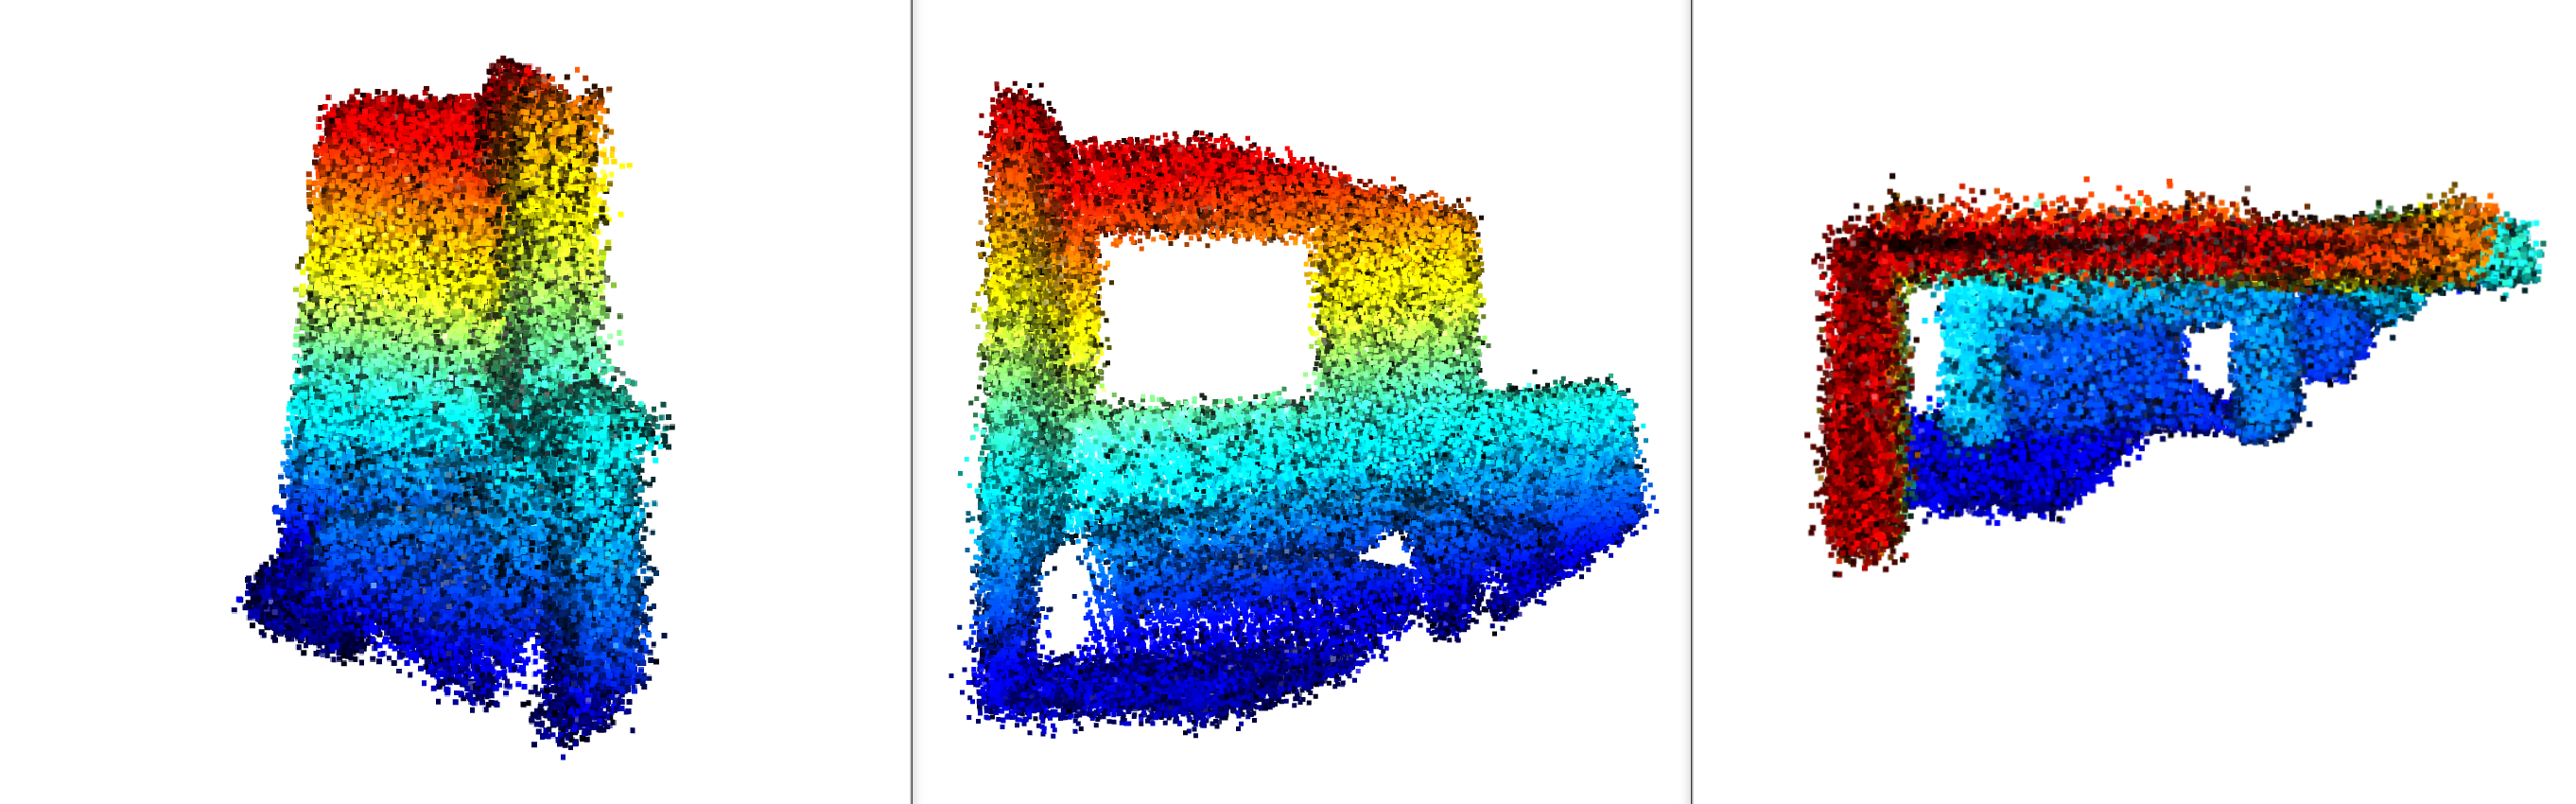
\includegraphics[width=1\textwidth]{noisy_pcl.png}
  \caption{Imagen de una nube de puntos procesada por el nodo ''noisy\textunderscore cloud''.}
\end{figure}
En resumen, este nodo se encarga de transformar la nube de puntos original a un estado simulado más cercano a la realidad de un sensor.

\subsubsection{Cálculo de la localización}
La piedra angular de este proyecto se asienta sobre las bases de la localización. Si se conoce la posición desde la que se ha capturado una nube de puntos, 
es posible trasladarla hasta esa posición para, a posteriori, ir calculando el desplazamiento entre nubes y componiendo este desplazamiento sobre la pose 
existente, repitiendo así este proceso de forma iterativa e indefinida, siempre y cuando sea capaz de hacer buenas estimaciones de estos desplazamientos. \newline
Este es un proceso complejo que consta de varios componentes asociados que trabajan en sintonía para generar salidas de igual importancia a la pose, como 
es el propio mapa. En este caso, se centra la atención en el proceso que lleva a cabo el nodo de localización llamado ''localization\textunderscore node''. 
Este nodo se encargará de recibir la nube de puntos (con o sin ruido), procesarla y calcular, a través de esta y la información previa, una nueva pose del sistema, 
además de decidir si hay nueva información que añadir al mapa.

\paragraph{Conceptos clave:}
Este componente se construye alrededor de varios conceptos fundamentales para el correcto funcionamiento de este proyecto, entre ellos se encuentran los 
siguientes:
\begin{itemize}
  \item \textbf{Preprocesamiento de la nube de puntos}: Hay que tener en cuenta que las nubes de puntos, tal como son recibidas, pueden no estar en el formato 
  correcto para ser procesadas, pueden contener errores, estar incompletas o necesitar transformaciones como traslación o reducción del muestreo (reducción 
  del número de puntos agrupándolos en función de la distancia entre ellos). En nuestro caso, la mayoría de transformaciones de preprocesamiento que se aplican 
  son:
  \begin{itemize}
    \item \textbf{Transformación de formato}: Dado que las nubes de puntos son recibidas en formato ''PointCloud2'', para poder trabajar con ellas y usar librerías como
    Open3D\cite{Zhou2018}, es necesario transformarlas a un formato compatible con estas librerías. En nuestro caso, se convierten a
    ''open3d.geometry.PointCloud()'' para poder trabajar con ellas usando las librerías Open3D\cite{Zhou2018} que se usarán a lo largo del proceso. 
    \item \textbf{Submuestreo (Downsampling)}: Dado que el mapa con el que se trabaja tiene una resolución determinada, es necesario reducir la resolución de
    las nubes de puntos que se reciben para que esta coincida con la del mapa. Esto se hace para reducir la cantidad de puntos a procesar, lo que mejora la 
    eficiencia computacional y reduce el ruido. En nuestro caso, se usa un método de submuestreo basado en un voxel grid, donde se agrupan los puntos dentro 
    de celdas de un tamaño determinado (tamaño del voxel) y se reemplazan por un solo punto representativo (generalmente el centroide de los puntos en esa celda).
    \item \textbf{Eliminación de outliers}: Las nubes de puntos pueden contener puntos erróneos o aislados que no representan la realidad del entorno. Estos outliers 
    pueden ser causados por ruido en la captura, errores de medición o reflejos. La eliminación de outliers es crucial para mejorar la calidad de la nube de puntos y 
    la precisión de los cálculos posteriores. En nuestro caso, se usa un método basado en la distancia media a los vecinos más cercanos, donde se eliminan los puntos 
    que están demasiado lejos de sus vecinos. Este proceso se realiza después del submuestreo para evitar eliminar puntos que podrían ser relevantes en la nube original.
    \item \textbf{Traslación al origen}: Las nubes de puntos capturadas suelen estar referenciadas a un sistema de coordenadas distinto al origen (0,0,0). Para facilitar 
    el cálculo del desplazamiento entre nubes y su emparejamiento con la nube anterior, es necesario trasladarlas al sistema de coordenadas del origen. Esto permite 
    que las transformaciones posteriores sean más consistentes y precisas.
    \item \textbf{Cálculo de normales}: El cálculo de las normales de los puntos en la nube es esencial para muchos algoritmos de procesamiento de nubes de puntos,
    incluyendo el emparejamiento ICP. Las normales proporcionan información sobre la orientación de las superficies representadas por la nube de puntos, lo que ayuda a 
    mejorar la precisión del emparejamiento. En nuestro caso, se calcula la normal de cada punto en función de sus vecinos más cercanos, usando un método basado en la
    covarianza local.
    \begin{figure}[h]
      \centering
        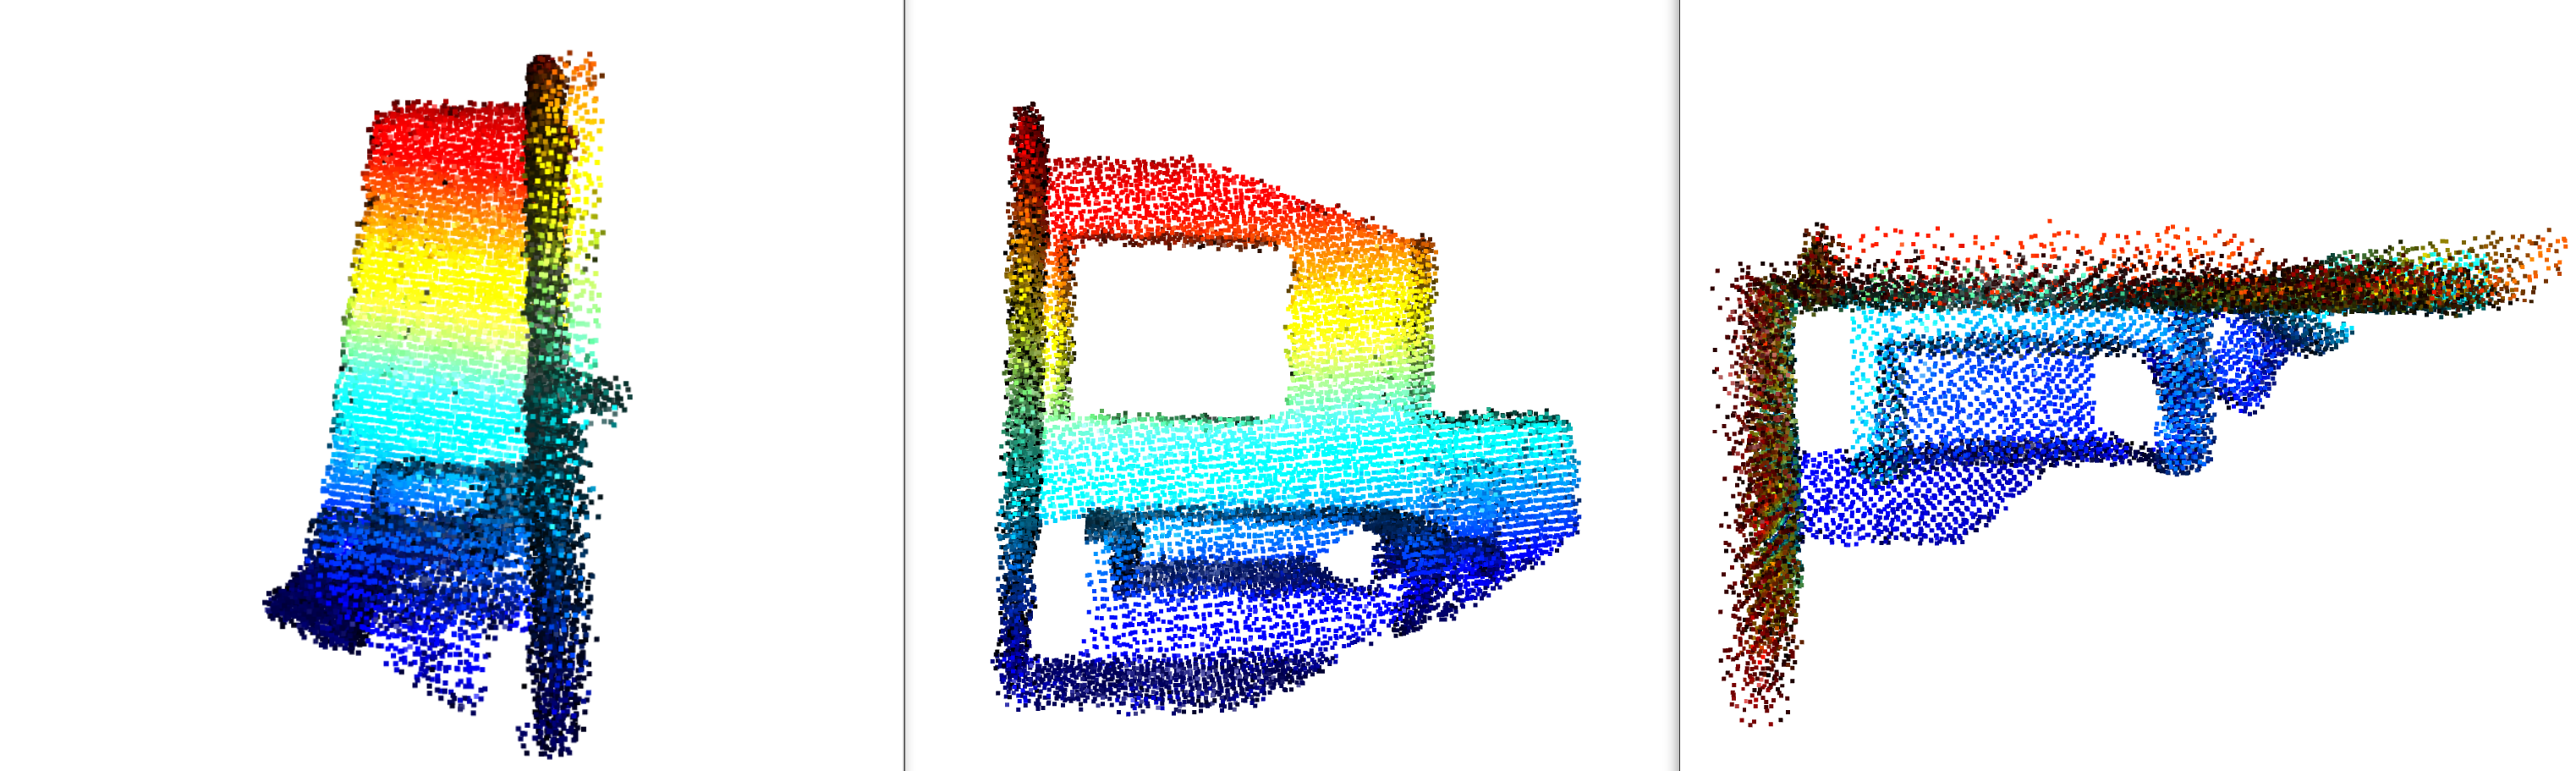
\includegraphics[width=1\textwidth]{preprocessed_pcl.png}
      \caption{Imagen de una nube de puntos procesada por la función de preprocesamiento.}
        \end{figure}
      \end{itemize}
      \item \textbf{ICP (Iterative Closest Point)}: El algoritmo \textit{Iterative Closest Point} (ICP) es un método ampliamente utilizado para la alineación de nubes de puntos 
      en aplicaciones de visión por computadora, robótica y reconstrucción 3D. Su objetivo es encontrar la transformación rígida óptima (rotación y traslación) que minimice la 
      distancia entre dos conjuntos de puntos: una nube de puntos \textit{fuente} $\mathcal{P} = \{\mathbf{p}_i\}_{i=1}^{N}$ y una nube de puntos \textit{objetivo} 
      $\mathcal{Q} = \{\mathbf{q}_j\}_{j=1}^{M}$, siendo \textit{N} y \textit{M} el número de puntos de cada una, respectivamente. A continuación, se describe su formulación matemática y el algoritmo paso a paso.
      \begin{itemize}
        \item \textbf{Formulación matemática}: El problema se modela como la búsqueda de una transformación rígida $(\mathbf{R}, \mathbf{t})$, donde $\mathbf{R} \in SO(3)$ es 
        una matriz de rotación y $\mathbf{t} \in \mathbb{R}^3$ es un vector de traslación, que minimice la siguiente función de costo:
    \[
    \min_{\mathbf{R}, \mathbf{t}} \; 
    E(\mathbf{R}, \mathbf{t}) =
    \frac{1}{|\mathcal{C}|} \sum_{(i,j) \in \mathcal{C}}
    \left\| \mathbf{q}_j - \big(\mathbf{R}\mathbf{p}_i + \mathbf{t}\big) \right\|^2
    \]
    donde $\mathcal{C}$ es el conjunto de correspondencias entre puntos de $\mathcal{P}$ y $\mathcal{Q}$ determinado en cada iteración.  
    
    \item \textbf{Algoritmo}: El procedimiento estándar de ICP consiste en los siguientes pasos iterativos:
    
    \begin{enumerate}
      \item \textbf{Inicialización:} Se establece una estimación inicial de la transformación $(\mathbf{R}_0, \mathbf{t}_0)$, que puede ser la identidad si no se dispone 
      de información previa.
      \item \textbf{Correspondencia:} Para cada punto $\mathbf{p}_i$ en la nube fuente, se busca el punto más cercano $\mathbf{q}_j$ en la nube objetivo según la métrica 
      euclidiana:
      \[
      j = \arg\min_{k} \left\| \mathbf{q}_k - \big(\mathbf{R}\mathbf{p}_i + \mathbf{t}\big) \right\|
      \]
      formando así el conjunto de correspondencias $\mathcal{C}$.
      \item \textbf{Optimización:} Se resuelve el problema de mínimos cuadrados para encontrar la nueva transformación $(\mathbf{R}, \mathbf{t})$ que minimice el error 
      cuadrático medio sobre las correspondencias. La solución cerrada se obtiene usando el método de Umeyama o descomposición en valores singulares (SVD):
      \begin{enumerate}
      \item Calcular los centroides de los puntos emparejados:
        \[
        \bar{\mathbf{p}} = \frac{1}{|\mathcal{C}|} \sum_{(i,j) \in \mathcal{C}} \mathbf{p}_i,
        \qquad
        \bar{\mathbf{q}} = \frac{1}{|\mathcal{C}|} \sum_{(i,j) \in \mathcal{C}} \mathbf{q}_j
        \]
        \item Construir la matriz de correlación:
        \[
        \mathbf{H} = \sum_{(i,j) \in \mathcal{C}}
        (\mathbf{p}_i - \bar{\mathbf{p}})
        (\mathbf{q}_j - \bar{\mathbf{q}})^{T}
        \]
        \item Obtener $\mathbf{R}$ y $\mathbf{t}$ mediante SVD:
        \[
        \mathbf{H} = \mathbf{U} \mathbf{\Sigma} \mathbf{V}^{T}
        \quad \Rightarrow \quad
        \mathbf{R} = \mathbf{V} \mathbf{U}^{T},
        \qquad
        \mathbf{t} = \bar{\mathbf{q}} - \mathbf{R}\bar{\mathbf{p}}
        \]
      \end{enumerate}
      \item \textbf{Transformación:} Actualizar la nube fuente aplicando la transformación obtenida.
      \item \textbf{Convergencia:} Repetir los pasos anteriores hasta que el cambio en el error $E(\mathbf{R}, \mathbf{t})$ entre iteraciones esté por debajo de un umbral 
      $\varepsilon$ o se alcance el número máximo de iteraciones.
        \end{enumerate}
        \item \textbf{Variantes de ICP:} Existen variantes que mejoran la robustez y velocidad del algoritmo, entre ellas:
        \begin{itemize}
      \item \textbf{ICP punto a punto (Point-to-Point):} Minimiza la distancia euclidiana entre puntos correspondientes (como en la formulación anterior).
      \item \textbf{ICP punto a plano (Point-to-Plane):} Minimiza la distancia entre el punto transformado y el plano tangente en $\mathbf{q}_j$, lo que conduce a una 
      convergencia más rápida:
      \[
      E(\mathbf{R}, \mathbf{t}) =
      \frac{1}{|\mathcal{C}|} \sum_{(i,j) \in \mathcal{C}}
      \left( \mathbf{n}_j^{T} \big(\mathbf{q}_j - (\mathbf{R}\mathbf{p}_i + \mathbf{t}) \big) \right)^{2}
      \]
      donde $\mathbf{n}_j$ es el vector normal asociado a $\mathbf{q}_j$.
        \end{itemize}
        \item \textbf{Implementación en Open3D\cite{Zhou2018}:} La librería \textit{Open3D}\cite{Zhou2018} proporciona una implementación optimizada de ICP en C++\cite{cpp} y Python\cite{python}. Su función principal para ello,
        \textit{registration\_icp()}, permite elegir entre varias métricas de alineación y utiliza aceleradores de búsqueda de vecinos como KD-Trees para obtener correspondencias eficientes.
        Además, Open3D\cite{Zhou2018} admite:
        \begin{itemize}
        \item \textbf{Jerarquía multiescala:} Aplicación de ICP en niveles de resolución decreciente para mejorar la convergencia global.
        \item \textbf{Criterios de parada:} Tolerancia de convergencia en función de la reducción relativa del error y límite de iteraciones.
        \item \textbf{Transformación inicial:} Opción de especificar $(\mathbf{R}_0, \mathbf{t}_0)$ para mejorar los resultados cuando se dispone de una estimación previa.
        \end{itemize}
      \end{itemize}

      \begin{figure}[h]
        \centering
      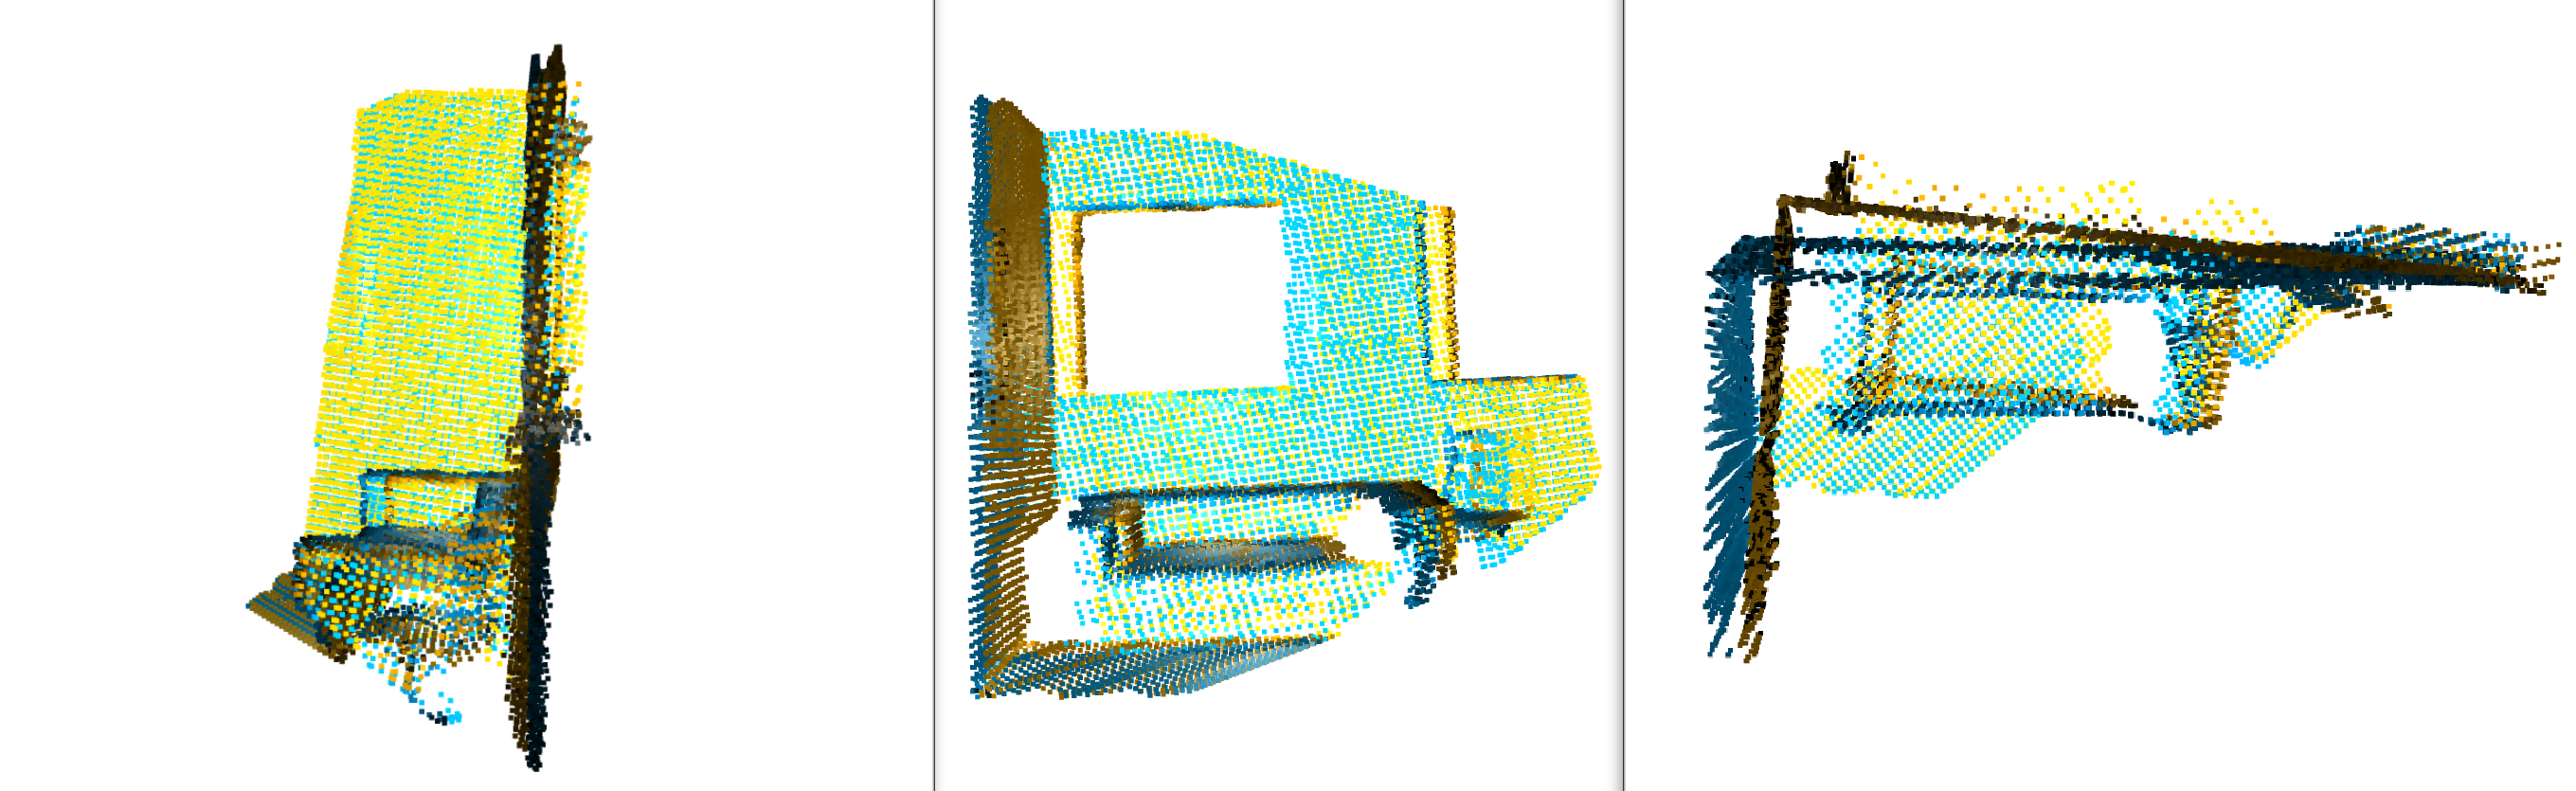
\includegraphics[width=1\textwidth]{misaligned_frames.png}
        \caption{Imagen de dos nubes de puntos desalineadas.}
      \end{figure}

      \begin{figure}[h]
        \centering
      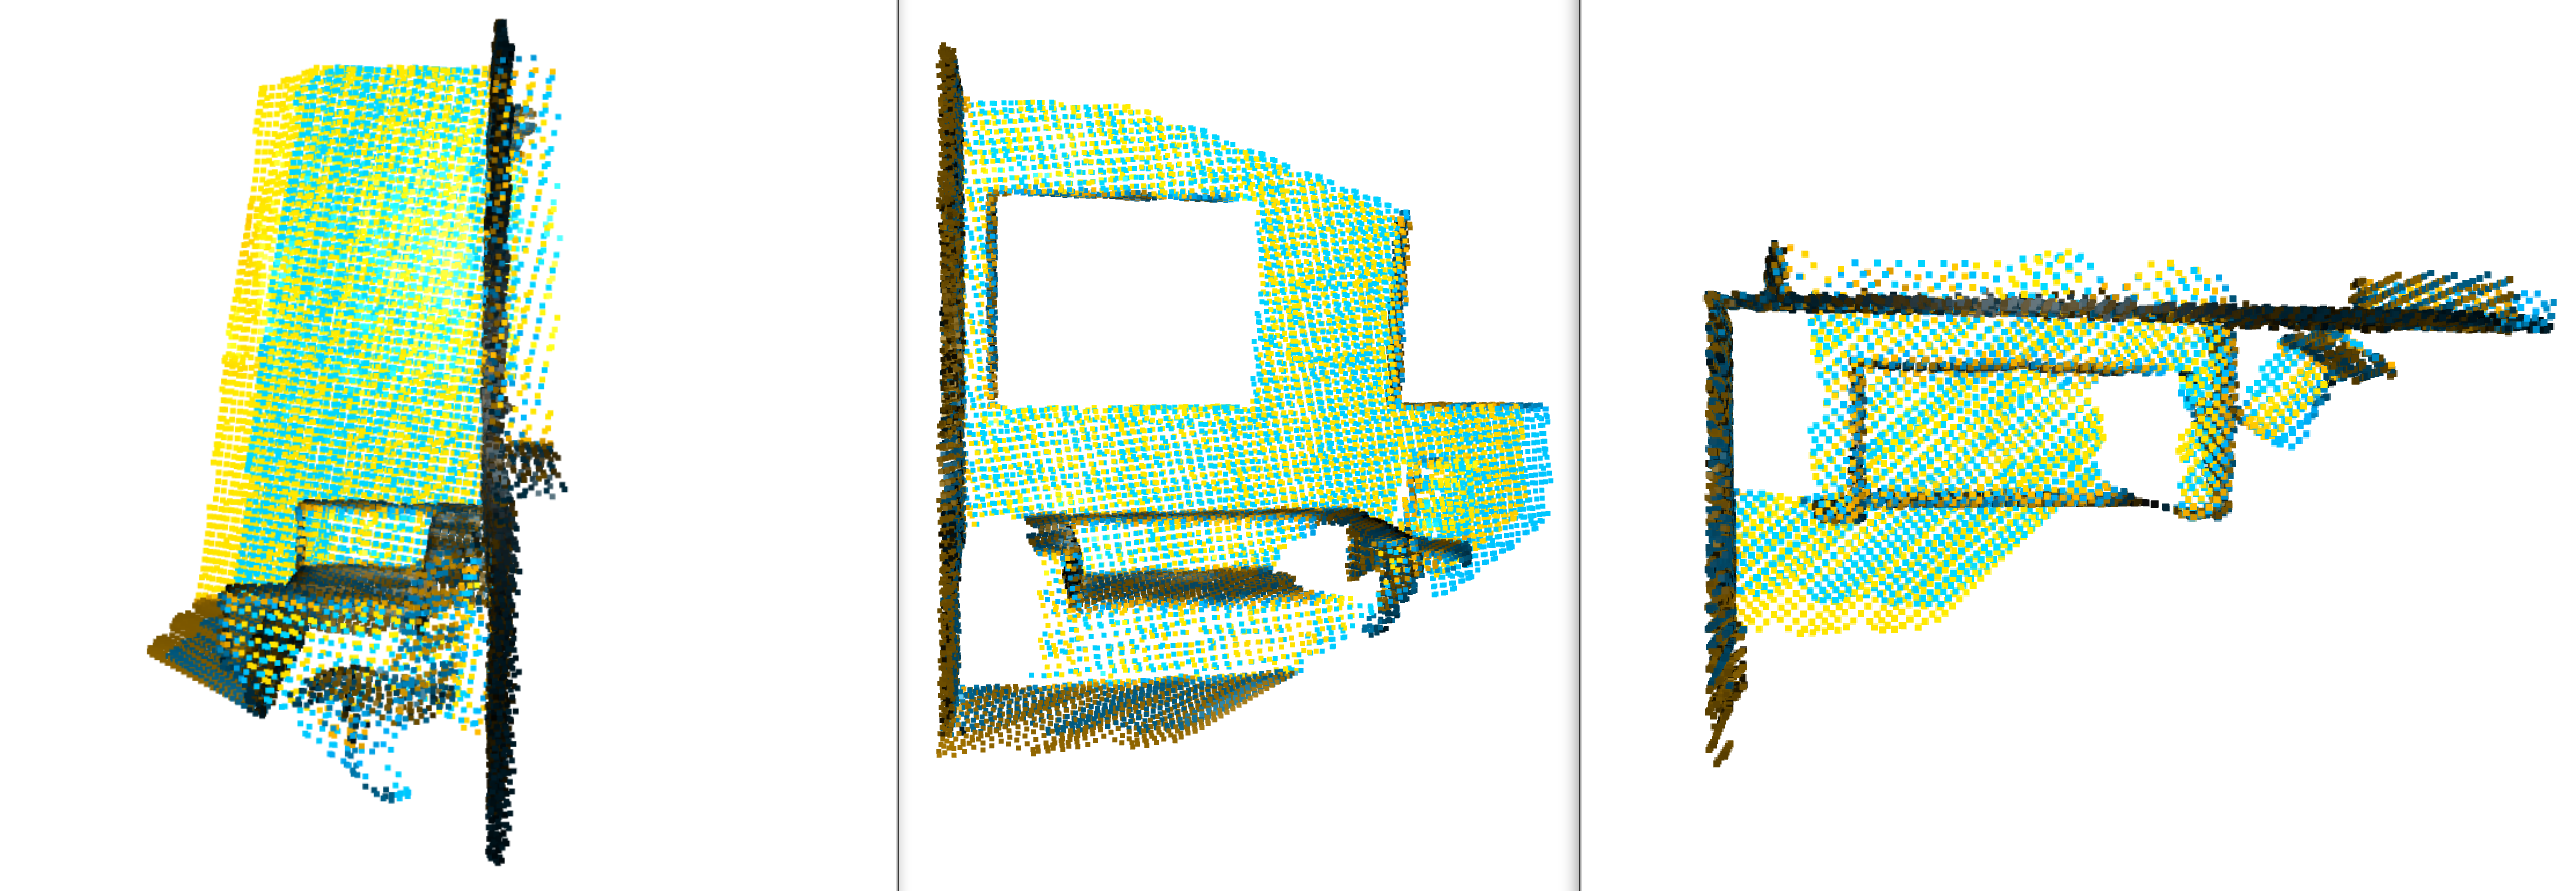
\includegraphics[width=1\textwidth]{aligned_frames.png}
        \caption{Imagen de dos nubes de puntos alineadas.}
      \end{figure} 

  \item \textbf{Selección de fotogramas clave (Key frame selection)}: El principio fundamental de la técnica de emparejamiento que se usa en este proyecto (ICP), al ser un método estadístico, es que siempre va a contener un mínimo de error.
  Aunque este error sea mínimo, si se va acumulando con el tiempo, puede llegar a corromper la pose y que esta deje de representar la realidad. Por ello, es necesario un proceso
  de curado y selección de fotogramas que construyan el mapa. Este proceso debe ser riguroso ya que, si se aceptan muchas nubes de puntos, el error se acumulará más rápidamente y, 
  si se aceptan pocas, el mapa será pobre, no representará la realidad y hará más complicado que se encuentren emparejamientos entre la nube actual y el mapa. \newline
  En este caso, se debe distinguir entre dos tipos de fotogramas clave:
  \begin{itemize}
    \item \textbf{Fotogramas clave para la localización}: Estos fotogramas clave son aquellos que se usan para mantener una referencia más actual de la pose 
    respecto del mapa, es decir, para reanclar la pose y evitar que el error se acumule demasiado. Para que uno de los fotogramas actuales sea considerado
    como fotograma clave para la localización, debe cumplir al menos una de las siguientes condiciones:
    \begin{itemize}
      \item \textbf{Distancia mínima desde la última clave}: Se define una distancia mínima que la nueva nube de puntos debe tener respecto a la última nube clave añadida al mapa.
      Esto asegura que las nubes de puntos añadidas al mapa estén suficientemente separadas espacialmente, lo que ayuda a cubrir más área del entorno y reduce la redundancia.
      Matemáticamente, si $\mathbf{p}_{\text{new}}$ es el centroide de la nueva nube de puntos y $\mathbf{p}_{\text{last}}$ es el centroide de la última nube clave, se requiere que:
      \[
      \|\mathbf{p}_{\text{new}} - \mathbf{p}_{\text{last}}\| > d_{\text{min}}
      \]
      donde $d_{\text{min}}$ es la distancia mínima requerida.
      \item \textbf{Cambio angular mínimo}: Se establece un umbral de cambio angular que la nueva nube de puntos debe superar respecto a la última nube clave. Esto garantiza que las 
      nubes de puntos se capturen desde diferentes orientaciones, lo que mejora la diversidad de perspectivas en el mapa.
      Matemáticamente, si $\mathbf{R}_{\text{new}}$ y $\mathbf{R}_{\text{last}}$ son las matrices de rotación asociadas a las nubes, el cambio angular $\theta$ se calcula como:
      \[
      \theta = \arccos\left(\frac{\text{trace}(\mathbf{R}_{\text{new}} \mathbf{R}_{\text{last}}^\top) - 1}{2}\right)
      \]
      y se requiere que $\theta > \theta_{\text{min}}$, donde $\theta_{\text{min}}$ es el umbral mínimo de cambio angular.
    \end{itemize}
    \item \textbf{Fotogramas clave para la construcción del mapa}: Estos fotogramas clave son aquellos que se usan para construir el mapa, es decir, para añadir nueva información
    al mapa. Para que uno de los fotogramas actuales sea considerado como fotograma clave para la construcción del mapa, debe cumplir al menos una de las siguientes condiciones:
    \begin{itemize}
      \item \textbf{Ratio de novedad mínimo}: Se calcula el ratio de novedad (información que aporta) entre la nueva nube de puntos y el mapa existente. Si este ratio es alto, 
      significa que la nueva nube aporta información significativa al mapa y, por tanto, debe ser añadida.
      Matemáticamente, si $N_{\text{overlap}}$ es el número de puntos de la nueva nube que coinciden con el mapa y $N_{\text{total}}$ es el número total de puntos en la nueva nube, el ratio de novedad $r$ se define como:
      \[
      r = 1-\frac{N_{\text{overlap}}}{N_{\text{total}}}
      \]
      y se requiere que $r > r_{\text{max}}$, donde $r_{\text{max}}$ es el umbral mínimo permitido.
    \end{itemize}
  \end{itemize}
\end{itemize}
\paragraph{Funcionamiento del componente:}
Tal y como se ha ido introduciendo, el nodo ''localization\textunderscore node'' se encargará de orquestar una serie de tareas cruciales que conciernen tanto 
a la localización global como a la construcción del mapa, por lo que detallar los pasos que este sigue es clave para comprender el funcionamiento de la herramienta. 
A continuación, se describen los pasos que sigue:
\begin{itemize}
  \item \textbf{Inicialización}: La inicialización de este nodo está conformada por los siguientes pasos:
  \begin{itemize}
    \item \textbf{Inicialización de publicadores y suscriptores}: Al instanciar el nodo, se inicia la escucha y se prepara para la recepción de mensajes de los 
    siguientes tópicos:
    \begin{itemize}
      \item \textbf{Suscripción de ''clean\textunderscore pcl'' o ''noisy\textunderscore cloud''}: Este suscriptor se encargará de recibir los mensajes de tipo 
      ''PointCloud2'' conteniendo la nube de puntos original o con ruido, en función del tipo de ejecución que hayamos decidido realizar.
      \item \textbf{Publicación de ''new\textunderscore pose''}: Este servicio de publicación se encarga de publicar mensajes de tipo ''PoseStamped'' conteniendo 
      la pose actualizada calculada a través de la última información recibida.
      \item \textbf{Publicación de ''new\textunderscore pcl''}: Este servicio de publicación se encarga de publicar mensajes de tipo ''PointCloud2'' conteniendo 
      la nube de puntos actualizada calculada a través de la última información recibida.
    \end{itemize}
    \item \textbf{Lectura del archivo de configuración}: Es necesario leer un archivo de configuración de tipo YAML\cite{yaml} que contiene los parámetros de evaluación de 
    algunas condiciones, parámetros de ICP, entre otros.
    \item \textbf{Inicialización de variables auxiliares para la ejecución}: Por último, se inicializarán algunas variables auxiliares como índices, entre otras, necesarias 
    para la correcta ejecución del nodo.
  \end{itemize}
   \item \textbf{Respuestas provocadas por la recepción de mensajes a través del tópico ''clean\textunderscore pcl'' o ''noisy\textunderscore pcl''}:
    Los mensajes recibidos por los tópicos de ''clean\textunderscore pcl'' o ''noisy\textunderscore pcl'' son la única entrada que no se genera de forma recursiva por 
    la ejecución del nodo, pero no es el único input usado. La ejecución de esta función se puede dividir en dos casos:
    \begin{itemize}
      \item \textbf{Primera llamada:} La primera llamada de este nodo se usa para inicializar una serie de elementos:
      \begin{itemize}
        \item \textbf{Almacenamiento de la primera nube de puntos:} Como este algoritmo usará dos nubes de puntos (''t-1'' y ''t'') para calcular el desplazamiento, en 
        la primera llamada no se dispone de ninguna nube previa, por lo que únicamente se llevará a cabo un preprocesamiento. \newline Aquí se transforma desde el tipo ''PointCloud2'' a 
        ''open3d.geometry.PointCloud()'', se realizará un submuestreo para igualar su resolución a la que usa el mapa, se hace una limpieza de outliers, se trasladará al 
        punto [x=0, y=0, z=0] y se calcularán sus normales, que son necesarias para realizar ICP, dejándola así lista para el siguiente paso.
        \item \textbf{Almacenamiento del primer fotograma clave y del mapa:} Dado que es la primera nube de puntos, servirá de punto de referencia, su pose 
        será el punto de origen, por lo que se puede usar como inicialización para el fotograma clave y el mapa.
        \item \textbf{Reconstrucción del mensaje y publicación:} Dado que en esta fase no hay ningún emparejamiento que calcular, solo se transforma la nube de puntos 
        de vuelta al tipo ''PointCloud2'' y se publica a través del tópico ''new\textunderscore pcl'' para que sea recibida por el módulo de mapeo.
      \end{itemize}
      \item \textbf{Llamadas sucesivas:} El resto de mensajes recibidos se tratarán de igual manera y siguiendo este esquema:
      \begin{itemize}
        \item \textbf{Preprocesamiento:} La nube de puntos se preprocesa de la misma manera que en el caso de la primera llamada, aunque se mantiene la copia original en 
        caso de que se requiera usar para el proceso de selección de nubes clave. Es decir, la nube se transforma desde el tipo ''PointCloud2'' a 
        ''open3d.geometry.PointCloud()'', se realiza el submuestreo a la resolución del mapa, se hace limpieza de outliers, se traslada a la pose calculada anteriormente y 
        se calculan las normales para poder realizar el posterior emparejamiento por ICP.
        \item \textbf{Lógica ICP:} Esta es la lógica principal, encargada de suministrar la nueva pose y nube de puntos trasladada a esa posición. Para implementar esta 
        lógica, se ha creado una función llamada ''icp\textunderscore logic'' que sigue el siguiente esquema:
        \begin{itemize}
          \item \textbf{Evaluación de emparejamiento fotograma a fotograma:} En primer lugar, se evalúa si debe realizarse un emparejamiento entre la nube actual y la
          nube anterior. La condición principal para que se realice este emparejamiento es que no haya pasado mucho tiempo desde la última vez que se encontró un nuevo fotograma clave.
          Esta es la condición a evaluar:
          \[
          (\text{Índice} - \text{Última\_ actualización}) \bmod \text{Umbral} = 0
          \]
          Si esta condición se cumple, se realiza el emparejamiento entre la nube actual y la anterior usando ICP punto a plano. Si el emparejamiento cumple todas las siguientes condiciones: \newline
          \textbf{Fitness > Umbral mínimo}\newline
          \textbf{RMSE < Umbral máximo}\newline
          \textbf{Distancia < Umbral máximo}\newline
          \textbf{Ángulo < Umbral máximo}\newline
          Entonces se actualiza y devuelve la pose, y el mapa vacío (ya que no pertenece al grupo de fotogramas que cumple las condiciones) y se almacena la nube actual como la nueva nube anterior.
          En caso de que no se cumpla alguna de las condiciones, se pasa a comprobar si es un fotograma clave.
          \item \textbf{Evaluación de fotograma clave:} Si la evaluación anterior no ha cumplido alguna de las condiciones, se intenta realizar un emparejamiento entre la nube actual y 
          el último fotograma clave. Si este emparejamiento cumple alguna de las siguientes condiciones:\newline
          \textbf{Distancia > Umbral mínimo}\newline
          \textbf{Ángulo > Umbral mínimo}\newline
          Si se ha cumplido alguna de las condiciones, este emparejamiento resulta en una nueva pose y fotograma clave. Además, se considera la posibilidad de que esta nube aporte
          nueva información al mapa, por lo que se evalúa si cumple la siguiente condición:\newline
          \textbf{Ratio de novedad > Umbral mínimo}\newline 
          Si se cumple esta condición, se devuelve la nueva pose y la nube actual para que sea añadida al mapa. En caso de que no se cumpla, se devuelve la nueva pose y un mapa vacío.
        \end{itemize}
        \item \textbf{Guardado de la nueva pose y publicación de la nueva información del mapa:} Una vez terminada la lógica de ICP, si se ha obtenido un nuevo fotograma clave perteneciente 
        al mapa, entonces este se publica y se esperará a la recepción del mapa actualizado para publicar la nueva pose. En caso contrario, se publica únicamente la nueva pose.
      \end{itemize}
    \end{itemize}
    \item \textbf{Respuestas provocadas por la recepción de mensajes a través del tópico \newline ''bonxai\_point\_cloud\_centers''}:
    Recibir un mensaje a través de este tópico significa que el mapa ha sido actualizado y, por tanto, se debe almacenar en el formato correcto, calcular sus normales y proceder 
    a publicar la nueva pose.
  \end{itemize}
 
\subsubsection{Construcción del mapa}
El mapeo es un componente esencial en aplicaciones de robótica y visión por computadora, donde la representación eficiente y precisa del entorno 3D es crucial.
En este contexto, las nubes de puntos seleccionadas como fotogramas clave se integran en una estructura de datos que permite almacenar y consultar información espacial 
de manera eficiente. Para este propósito, se ha diseñado un nodo llamado ''mapping\textunderscore node'' que utiliza la biblioteca \textit{Bonxai}\cite{faconti2024bonxai} para gestionar el mapa 3D.
\textit{Bonxai}\cite{faconti2024bonxai} es una biblioteca de código abierto diseñada para la representación, manipulación y consulta eficiente de datos volumétricos en 3D mediante una estructura 
jerárquica y dispersa de tipo \textit{Voxel Grid}. Su objetivo es proporcionar una alternativa moderna y de alto rendimiento a bibliotecas como \textit{Octomap}, 
manteniendo soporte para entornos de tamaño ilimitado (\textit{unbounded}), almacenamiento eficiente de memoria y tiempos de acceso rápidos.\newline
La estructura de datos de Bonxai\cite{faconti2024bonxai} permite representar el espacio 3D como una colección de celdas cúbicas (voxels) de tamaño uniforme \(\Delta \in \mathbb{R}^{+}\), 
organizadas jerárquicamente para garantizar eficiencia en memoria y operaciones. Esta característica lo hace especialmente útil en aplicaciones de mapeo y localización en robótica, 
donde la representación del entorno debe ser consistente, escalable y fácilmente actualizable.

\paragraph{Conceptos clave:}
Los conceptos fundamentales que sustentan la construcción del mapa son conceptos intrínsecos del funcionamiento de Bonxai\cite{faconti2024bonxai}, siendo estos los siguientes:
\begin{itemize}
  \item \textbf{Voxel Grid jerárquico}:  
  El espacio continuo \(\mathbb{R}^{3}\) se discretiza en una cuadrícula regular de vóxeles con resolución \(\Delta\).  
  Cada punto del espacio \(\mathbf{x} = (x,y,z) \in \mathbb{R}^{3}\) se asigna a un vóxel mediante:
  \[
  \mathrm{coord}(\mathbf{x}) = \left( 
  \left\lfloor \frac{x}{\Delta} \right\rfloor,\ 
  \left\lfloor \frac{y}{\Delta} \right\rfloor,\ 
  \left\lfloor \frac{z}{\Delta} \right\rfloor
  \right) \in \mathbb{Z}^{3}
  \]
  donde cada coordenada entera representa un índice de vóxel.  
  Esta discretización define una partición del espacio:
  \[
  \mathbb{R}^{3} = \bigcup_{\mathbf{k} \in \mathbb{Z}^{3}} V_{\mathbf{k}}, \quad
  V_{\mathbf{k}} = \{\mathbf{x} \in \mathbb{R}^{3} : \mathrm{coord}(\mathbf{x}) = \mathbf{k}\}
  \]
  donde \(V_{\mathbf{k}}\) es la celda cúbica asociada al índice \(\mathbf{k}\).
  \item \textbf{Estructura jerárquica y dispersa}:  
  Los vóxeles se almacenan de forma dispersa usando un árbol jerárquico, donde únicamente las celdas activas (ocupadas o modificadas) se mantienen en memoria.  
  Esto permite que el costo de almacenamiento sea proporcional al número de celdas activas \(N\):
  \[
  \mathcal{O}(\text{memoria}) = \mathcal{O}(N)
  \]
  en lugar de depender del volumen total del espacio explorado.
  \item \textbf{Acceso eficiente mediante Accessor}:  
  Bonxai\cite{faconti2024bonxai} proporciona un objeto \textit{Accessor} que permite acceso de lectura/escritura en tiempo cercano a \(\mathcal{O}(1)\) para operaciones de inserción, actualización y 
  consulta:
  \[
  \text{setValue}: \mathbf{k} \mapsto v, \qquad
  \text{value}: \mathbf{k} \mapsto v \ \text{o} \ \varnothing
  \]
  donde \(v \in T\) es el valor almacenado (por ejemplo, probabilidad de ocupación, intensidad de un sensor, etc.).
  \item \textbf{Almacenamiento de datos personalizados}:  
  Cada vóxel puede almacenar un tipo de dato arbitrario \(T\), lo que permite utilizar Bonxai\cite{faconti2024bonxai} no solo para mapas de ocupación binaria, sino también para mapas de distancia firmada 
  (ESDF), probabilidades bayesianas de ocupación, valores de intensidad o información semántica.
  \item \textbf{Escalabilidad y precisión}:  
  La resolución \(\Delta\) se elige según la aplicación. Con coordenadas enteras de 32 bits, el rango máximo por eje es:
  \[
  R_{\max} = 2^{32} \cdot \Delta
  \]
  lo que, para \(\Delta = 0.01\ \mathrm{m}\), cubre hasta \(\approx 42\ \mathrm{km}\) por eje, suficiente para la mayoría de aplicaciones robóticas en entornos extensos.
  \item \textbf{Operaciones principales}:  
  Además de inserción y consulta, Bonxai\cite{faconti2024bonxai} soporta iteración eficiente sobre los vóxeles activos:
  \[
  \text{IterateAllCells} : \{\mathbf{k}_1, \dots, \mathbf{k}_N\} \mapsto 
  \{(\mathbf{k}_i, v_i)\}_{i=1}^{N}
  \]
  lo que permite exportar, serializar o realizar operaciones globales sobre el mapa.
\end{itemize}

\paragraph{Funcionamiento del componente:}
Bonxai\cite{faconti2024bonxai} se integra en el nodo ''mapping\textunderscore node'' a través de un componente facilitado por la propia librería llamado ''BonxaiServer'', que se encarga de gestionar
la estructura de datos y proporcionar una interfaz sencilla para interactuar con el mapa. El funcionamiento de este nodo se puede describir de la siguiente manera:
\begin{itemize}
  \item \textbf{Inicialización}: La inicialización de este nodo está conformada por los siguientes pasos:
  \begin{itemize}
    \item \textbf{Suscripción de ''new\textunderscore pcl''}: Este suscriptor se encargará de recibir los mensajes de tipo ''PointCloud2'' que contienen la nube de puntos 
    trasladada a la posición calculada por el algoritmo.
    \item \textbf{Inicialización del servidor Bonxai\cite{faconti2024bonxai}}: Se crea una instancia del servidor Bonxai\cite{faconti2024bonxai} como un componente al que se accede para gestionar el mapa.
  \end{itemize}
  \item \textbf{Respuestas provocadas por la recepción de mensajes a través del tópico ''new\textunderscore pcl''}:
  Los mensajes recibidos por el tópico ''new\textunderscore pcl'' iniciarán el proceso de integración de la nueva nube de puntos en el mapa. 
  La ejecución de esta función comprueba que el mensaje recibido no es nulo y, en caso de que no lo sea, se llama a la función proporcionada por el servidor Bonxai\cite{faconti2024bonxai}
  para integrar la nube de puntos en el mapa y, además, publicar el mapa actualizado a través de un tópico llamado ''bonxai\textunderscore point\textunderscore cloud\textunderscore centers''.
\end{itemize}

\subsection{Flujo de trabajo completo}
En esta sección se describe el flujo de trabajo completo, las salidas de cada uno de los componentes y las interacciones entre ellos. El flujo de trabajo completo del sistema de localización 
y mapeo se puede describir de la siguiente manera:
\begin{figure}[h]
  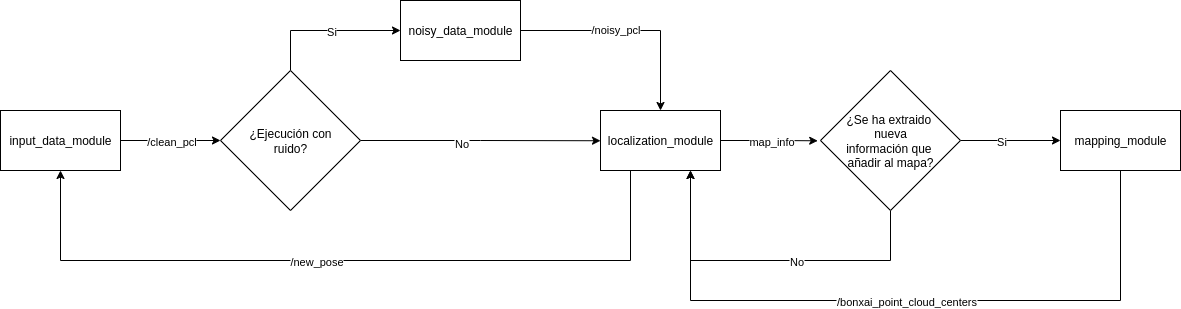
\includegraphics[width=1\textwidth]{Diagrama.png}
  \caption{Diagrama simplificado sobre las interacciones entre nodos.}
\end{figure}
\begin{enumerate}
  \item \textbf{Input\_data\_node:} Este nodo leerá una pose y una nube de puntos de la grabación y las publicará a través de los tópicos 
  ''clean\_pose'' y ''clean\_pcl'', respectivamente. Se quedará a la espera de que el nodo de localización publique la nueva pose para publicar 
  la siguiente pose y nube de puntos.
  \item \textbf{(Opcional) Noisy\_data\_node:} 
  Este nodo se ejecutará si se decide hacer una ejecución con ruido. En ese caso, interceptará los mensajes de ''clean\_pcl'', añadirá ruido y los publicará a través del tópico
  ''noisy\_pcl''. En caso contrario, este nodo no se ejecutará y el nodo de localización escuchará directamente los mensajes de ''clean\_pcl''.
  \item \textbf{Localization\_node:} Este nodo escuchará los mensajes de ''clean\_pcl'' o ''noisy\_pcl'' en función del tipo de ejecución. Cada vez que reciba una nube de puntos, 
  realizará el preprocesamiento y la lógica de ICP para calcular la nueva pose y decidir si la nube actual es un fotograma clave. Si el fotograma actual es clave y añade información 
  al mapa, publicará la nueva nube de puntos a través del tópico ''new\_pcl'' y esperará a que el nodo de mapeo publique el mapa actualizado para publicar la nueva pose.
  En caso de que el fotograma actual no sea clave, publicará la nueva pose a través del tópico ''new\_pose''.
  \item \textbf{Mapping\_node:} Este nodo escuchará los mensajes de ''new\_pcl''. Cada vez que reciba una nube de puntos, la integrará en el mapa usando Bonxai\cite{faconti2024bonxai} y publicará el mapa actualizado a través del tópico
  ''bonxai\_point\_cloud\_centers''. El nodo de localización escuchará este tópico para publicar la nueva pose.
\end{enumerate}


\section{Pruebas y validación de resultados}
La validación de los resultados obtenidos por el sistema de localización y mapeo es crucial para asegurar su precisión y fiabilidad en aplicaciones del mundo real. Para ello, se han diseñado y 
ejecutado una serie de pruebas que evalúan el rendimiento del sistema tanto a nivel de localización como de construcción del mapa. A continuación, se describen las métricas de interés en cada caso, 
metodologías empleadas, los escenarios de prueba y los resultados obtenidos.

\subsection{Métricas de interés}
Antes de comenzar a describir las pruebas realizadas, es importante definir las métricas clave que se utilizarán para evaluar el rendimiento del sistema. Además de esto, como se deben evaluar las dos 
salidas principales del sistema (pose y mapa), las métricas se dividen en dos categorías: métricas de localización y métricas de mapeo.

\subsubsection{Métricas de Evaluación de Localización}

En el contexto de \textit{SLAM} sin cierre de bucle, es fundamental cuantificar 
la precisión de la estimación de la trayectoria del robot a lo largo del tiempo. 
En esta sección se describen tres métricas ampliamente utilizadas: 
\textbf{Absolute Trajectory Error (ATE\cite{Chen2022DELOATE})}, 
\textbf{Relative Pose Error (RPE\cite{Sturm2012RPE})} y 
\textbf{KITTI-style Drift\cite{Geiger2013KITTI}}, incluyendo su formulación matemática, motivación y forma de interpretación. 
\newpage

\paragraph{Absolute Trajectory Error (ATE\cite{Chen2022DELOATE})}

\subparagraph{Definición matemática:}
Sea $\mathbf{T}^{gt}_i \in SE(3)$ la pose de referencia (ground-truth) en el instante $i$ 
y $\mathbf{T}^{est}_i \in SE(3)$ la pose estimada por el sistema SLAM\cite{smith1987slam}.
El ATE\cite{Chen2022DELOATE} mide el error de traslación absoluto después de alinear la trayectoria estimada 
con la de referencia mediante una transformación de similitud rígida $S \in Sim(3)$
(obtenida mediante un ajuste de mínimos cuadrados de tipo Horn o Umeyama):
\[
\text{ATE}_{rmse} = 
\sqrt{\frac{1}{N}\sum_{i=1}^{N} 
\left\| 
\mathrm{trans}\!\left(
(\mathbf{T}^{gt}_i)^{-1} \cdot (S \mathbf{T}^{est}_i)
\right)
\right\|^2 }
\]
donde $\mathrm{trans}(\cdot)$ extrae el vector de traslación de la transformación homogénea.

\subparagraph{Motivación:}
El ATE\cite{Chen2022DELOATE} evalúa el error acumulado de la trayectoria en coordenadas globales.
Es especialmente relevante en escenarios sin cierre de bucle porque 
revela de manera directa la \textbf{deriva acumulada} en posición a lo largo de la secuencia.

\subparagraph{Área de interés:}
\begin{itemize}
  \item Precisión global de localización.
  \item Consistencia con el sistema de referencia absoluto.
  \item Comparación directa de trayectorias completas.
\end{itemize}

\subparagraph{Interpretación:}
\begin{itemize}
  \item Valores bajos de ATE\cite{Chen2022DELOATE} indican que la trayectoria estimada está bien alineada con la de referencia.
  \item Un incremento progresivo de ATE\cite{Chen2022DELOATE} a lo largo del tiempo es indicativo de deriva acumulativa.
  \item El ATE\cite{Chen2022DELOATE} es sensible a errores de escala (en monocular SLAM\cite{smith1987slam}) y a falta de cierre de bucle.
\end{itemize}

\subparagraph{Resultados:}
Los resultados del ATE\cite{Chen2022DELOATE} se obtienen de comparar la trayectoria original (ground-truth) con la trayectoria estimada por el sistema de localización. 
Los resultados son los siguientes:
\begin{itemize}
  \item \textbf{Ejecición sin ruido:} Los valores obtenidos son:
  \begin{itemize}
    \item \textbf{ATE\cite{Chen2022DELOATE} (RMSE):} 0.319 metros.
    \item \textbf{ATE\cite{Chen2022DELOATE} mediana:}: 0.312 metros.
    \item \textbf{ATE\cite{Chen2022DELOATE} máximo:} 0.582 metros.
    \begin{figure}[h]
      \centering
        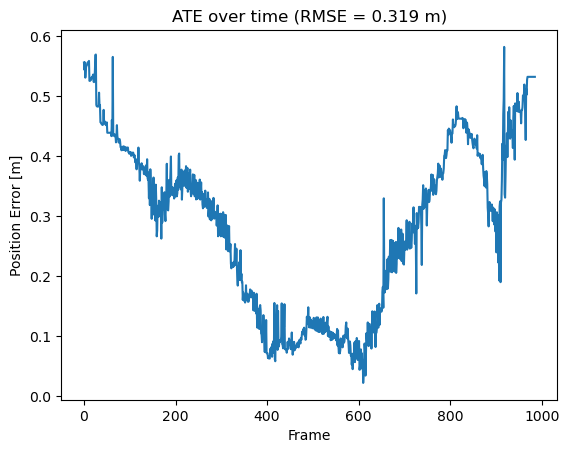
\includegraphics[width=0.3\textwidth]{ate_clean.png}
      \caption{Evolución del ATE\cite{Chen2022DELOATE} a lo largo de la ejecución.}
    \end{figure} 
  \end{itemize}
  \item \textbf{Ejecición con ruido:} Los valores obtenidos son:
  \begin{itemize}
    \item \textbf{ATE\cite{Chen2022DELOATE} (RMSE):} 0.314 metros.
    \item \textbf{ATE\cite{Chen2022DELOATE} mediana:}: 0.306 metros.
    \item \textbf{ATE\cite{Chen2022DELOATE} máximo:} 0.589 metros.
    \begin{figure}[h]
      \centering
        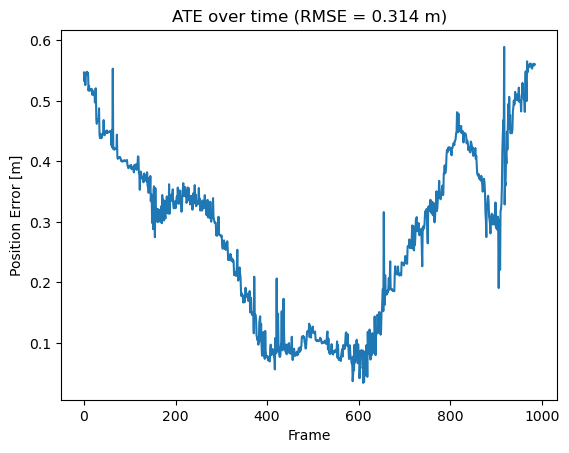
\includegraphics[width=0.3\textwidth]{ate_noisy.png}
      \caption{Evolución del ATE\cite{Chen2022DELOATE} a lo largo de la ejecución.}
    \end{figure} 
  \end{itemize}
\end{itemize}

\subparagraph{Interpretación de resultados:}
Los resultados obtenidos para el ATE\cite{Chen2022DELOATE} en ambas ejecuciones (con y sin ruido) son
sorprendentemente similares, con valores de RMSE alrededor de 0.31 metros.
Esto indica que el sistema de localización es robusto frente al ruido introducido,
manteniendo una precisión global consistente.\newline
La mediana del ATE\cite{Chen2022DELOATE} también es cercana al RMSE, lo que sugiere que
los errores no están dominados por unos pocos valores atípicos.
El ATE\cite{Chen2022DELOATE} máximo, ligeramente superior en la ejecución con ruido, refleja
algunos picos de error. Esto podría atribuirse, en parte, al ruido de la ejecución y 
a discontinuidades en la grabación, que no actualiza la pose en cada fotograma, sino
de forma asíncrona.\newline
Además, se puede ver cómo el gráfico contiene muchas pequeñas irregularidades. Esto se 
debe al anclaje con el fotograma clave, que hace que la trayectoria no sea completamente suave.
En conjunto, estos resultados demuestran que el sistema de localización
mantiene una buena precisión global incluso en presencia de ruido.


\paragraph{Relative Pose Error (RPE\cite{Sturm2012RPE})}

\subparagraph{Definición matemática:}
El RPE\cite{Sturm2012RPE} mide la consistencia local de la estimación de movimiento entre poses 
separadas por un intervalo temporal $\Delta t$.
Se define el error relativo entre la transformación de referencia y la estimada como:
\[
\mathbf{E}_i =
\left[
(\mathbf{T}^{gt}_i)^{-1}\mathbf{T}^{gt}_{i+\Delta}
\right]^{-1}
\cdot
\left[
(\mathbf{T}^{est}_i)^{-1}\mathbf{T}^{est}_{i+\Delta}
\right]
\]
La métrica RPE\cite{Sturm2012RPE} de traslación (en RMSE) se calcula como:
\[
\text{RPE}_{trans} =
\sqrt{\frac{1}{M}\sum_{i=1}^{M}
\|\mathrm{trans}(\mathbf{E}_i)\|^2 }
\]
donde $M$ es el número de pares válidos de poses.
De forma análoga, puede calcularse un error angular usando $\mathrm{rot}(\mathbf{E}_i)$.

\subparagraph{Motivación:}
El RPE\cite{Sturm2012RPE} mide la \textbf{precisión local del movimiento relativo}, 
independientemente de la deriva global.
En ausencia de cierre de bucle, el RPE\cite{Sturm2012RPE} es muy útil porque 
puede permanecer bajo incluso si la trayectoria global se ha desviado,
siempre que las estimaciones locales sean coherentes.
\subparagraph{Área de interés:}
\begin{itemize}
  \item Consistencia local de la odometría.
  \item Estabilidad de la integración incremental.
  \item Detección de saltos o discontinuidades en la estimación de pose.
\end{itemize}

\subparagraph{Interpretación:}
\begin{itemize}
  \item Valores bajos de RPE\cite{Sturm2012RPE} indican que la odometría es localmente coherente.
  \item Un RPE\cite{Sturm2012RPE} alto suele señalar errores en el cálculo de la transformación incremental 
  (por ejemplo, fallos en la estimación de ICP, ruido excesivo de sensores o reinicios de pose).
\end{itemize}

\subparagraph{Resultados:}
Los resultados del RPE\cite{Sturm2012RPE} se obtienen de comparar el movimiento relativo cada \textit{N} fotogramas entre la pose original (ground-truth) y la estimada por el sistema de localización. 
Los resultados son los siguientes:
\begin{itemize}
  \item \textbf{Ejecución sin ruido:} Los valores obtenidos son: \newline

  \begin{figure}[h]
    \centering
      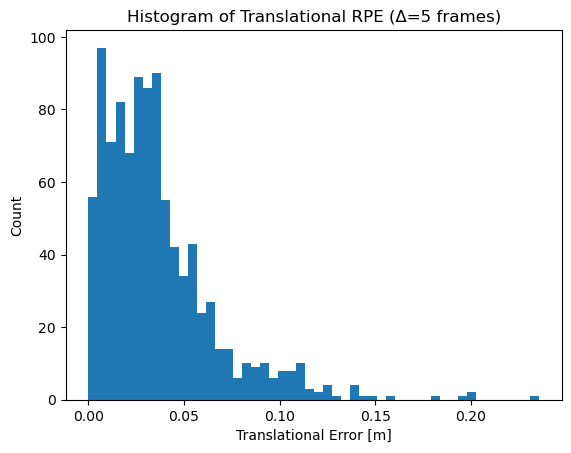
\includegraphics[width=0.4\textwidth]{rpe_clean.png}
    \caption{Distribución del error traslacional cada 5 frames en la ejecucion.}
  \end{figure} 
  \newpage

  \item \textbf{Ejecución con ruido:} Los valores obtenidos son: \newline

  \begin{figure}[h]
    \centering
      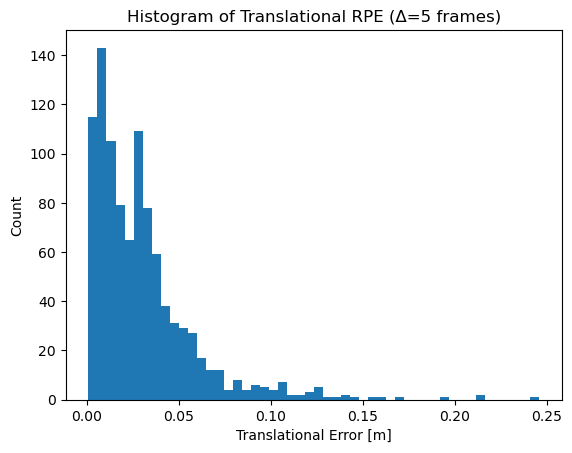
\includegraphics[width=0.4\textwidth]{rpe_noisy.png}
    \caption{Distribución del error traslacional cada 5 frames en la ejecucion.}
  \end{figure} 

\end{itemize}

\subparagraph{Interpretación de resultados:}
Los resultados del RPE\cite{Sturm2012RPE} muestran que el sistema de localización mantiene una buena consistencia local tanto en la ejecución sin ruido como en la ejecución con ruido.
En ambas ejecuciones, el RPE\cite{Sturm2012RPE} de traslación se mantiene en valores bajos, alrededor de 0,05 metros, lo que indica que las estimaciones de movimiento entre poses consecutivas
son precisas y coherentes.\newline
La ligera variación en el RPE\cite{Sturm2012RPE} entre las dos ejecuciones sugiere que el sistema es robusto frente al ruido, ya que la presencia de ruido no ha provocado un aumento significativo en
el error local.\newline

\paragraph{KITTI-style Drift\cite{Geiger2013KITTI}:}
\subparagraph{Definición matemática:}
En el benchmark KITTI\cite{Geiger2013KITTI}, la deriva se evalúa sobre tramos de longitud $L$ (p. ej. $L \in \{1,2, \dots,10\}$ metros).
Para cada segmento se calcula el error relativo de traslación y de rotación:
\[
\text{drift}(L) = 
\frac{1}{|S_L|} \sum_{s \in S_L}
\frac{\| \mathrm{trans}(\mathbf{E}_s)\|}{L}
\]
donde $S_L$ es el conjunto de todos los subtramos de longitud $L$ y 
$\mathbf{E}_s$ es el error relativo de pose en el subtramo.

\subparagraph{Motivación:}
Esta métrica ofrece una visión \textbf{normalizada por distancia recorrida} 
de la deriva, lo que permite comparar secuencias de distinta longitud.

\subparagraph{Área de interés:}
\begin{itemize}
  \item Tasa de acumulación de error por metro recorrido.
  \item Comparación con otros sistemas de odometría visual/SLAM\cite{smith1987slam} en datasets estándar.
  \item Identificación de segmentos de trayectoria con peor rendimiento.
\end{itemize}

\subparagraph{Interpretación:}
\begin{itemize}
  \item Un drift de traslación bajo (p. ej. $< 1\%$) indica que el sistema es robusto 
  y que la trayectoria estimada sigue de cerca la referencia en cada tramo.
  \item Un incremento del drift con $L$ es normal, pero un crecimiento excesivo 
  puede indicar que la integración de movimiento está acumulando error rápidamente.
\end{itemize}

\subparagraph{Resultados:}
Los resultados del KITTI\cite{Geiger2013KITTI} se obtienen de comparar segmentos de la pose original (ground-truth) con segmentos estimados por el sistema de localización y mapeo. 
Los resultados son los siguientes:
\begin{itemize}
  \item \textbf{Ejecución sin ruido:} Los valores obtenidos son:
  \begin{itemize}
    \item \textbf{Derrape traslacional, medio:} 3.15\%.
    \item \textbf{Derrape traslacional, mediana:} 3.21\%.
    \item \textbf{Derrape rotacional, medio:} 34º/100 metros.
    \begin{figure}[h]
      \centering
        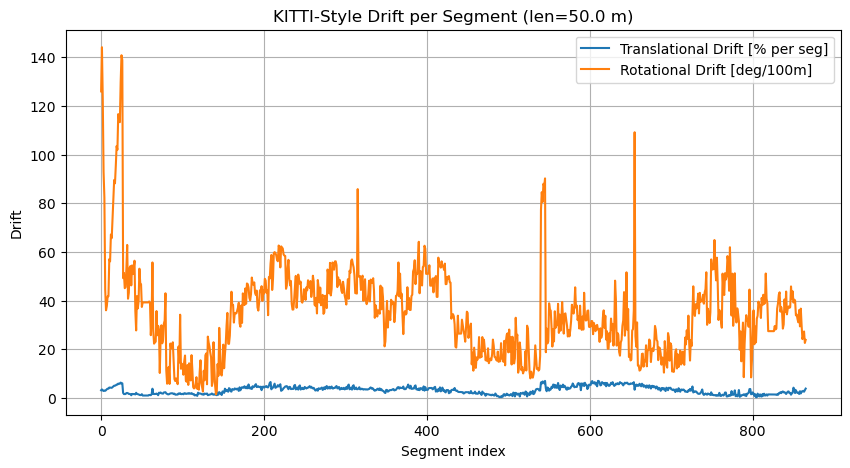
\includegraphics[width=0.4\textwidth]{kitty_clean.png}
      \caption{Evolución del KITTI\cite{Geiger2013KITTI} a lo largo de la ejecución.}
    \end{figure} 
    \end{itemize}
  \item \textbf{Ejecución con ruido:} Los valores obtenidos son:
  \begin{itemize}
    \item \textbf{Derrape traslacional, medio:} 4.13\%.
    \item \textbf{Derrape traslacional, mediana:} 4.22\%.
    \item \textbf{Derrape rotacional, medio:} 43º/100 metros.
    \begin{figure}[h]
      \centering
        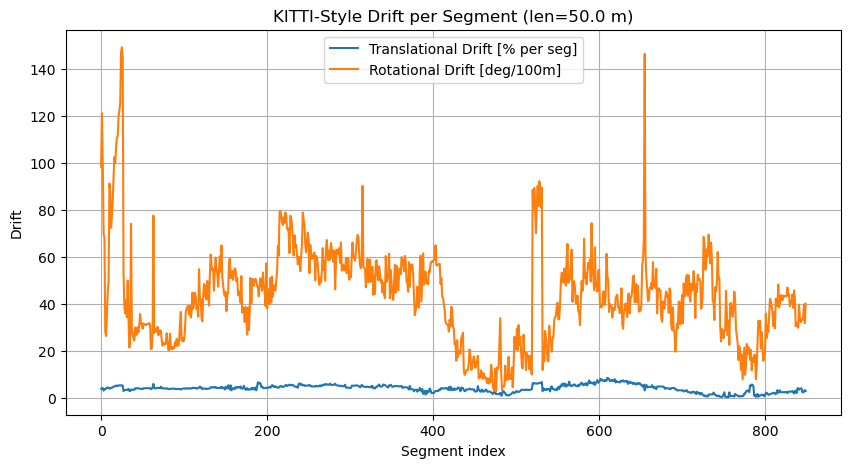
\includegraphics[width=0.4\textwidth]{kitty_noisy.png}
      \caption{Evolución del KITTI\cite{Geiger2013KITTI} a lo largo de la ejecución.}
    \end{figure} 
  \end{itemize}
\end{itemize}
\subparagraph{Interpretación de resultados:}
Los resultados del KITTI-style drift\cite{Geiger2013KITTI} indican que el sistema de localización y mapeo mantiene
una tasa de acumulación de error razonable en ambas ejecuciones (con y sin ruido).
En la ejecución sin ruido, el derrape traslacional medio es del 3.15\%, lo que sugiere que el sistema es capaz de seguir la trayectoria de referencia con una
precisión adecuada en cada tramo de 50 metros. La mediana cercana al valor medio indica
que los errores no están dominados por unos pocos segmentos atípicos.\newline
En la ejecución con ruido, el derrape traslacional medio aumenta a 4.13,\% lo que refleja el impacto del ruido en la precisión local.
Aunque hay un incremento, el valor sigue siendo aceptable, indicando que el sistema es robusto frente al ruido.
El derrape rotacional también muestra un aumento, pasando de 34º/100 metros a 43º/100 metros, lo que sugiere que el ruido afecta más a la estimación de orientación que
a la de posición.\newline

\paragraph{Resumen de métricas de localización}
En resumen, las métricas de localización (ATE, RPE y KITTI-style drift\cite{Geiger2013KITTI}) proporcionan una visión completa del rendimiento del sistema de localización y mapeo.
El ATE\cite{Chen2022DELOATE} revela la precisión global de la trayectoria, el RPE\cite{Sturm2012RPE} evalúa la consistencia local del movimiento y el KITTI-style drift\cite{Geiger2013KITTI} normaliza la deriva por distancia recorrida.
Los resultados obtenidos en ambas ejecuciones (con y sin ruido) demuestran que el sistema es robusto y mantiene una buena precisión tanto a nivel global como local, incluso en presencia de ruido.
Estas métricas son fundamentales para validar la eficacia del sistema en escenarios de SLAM\cite{smith1987slam} sin cierre de bucle. Además, haciendo una inspección visual de la trayectoria, se puede observar que el sistema sigue de manera bastante fiel la trayectoria original,
con pequeñas desviaciones que se corresponden con los errores cuantificados por las métricas.

\begin{figure}[h]
  \centering
    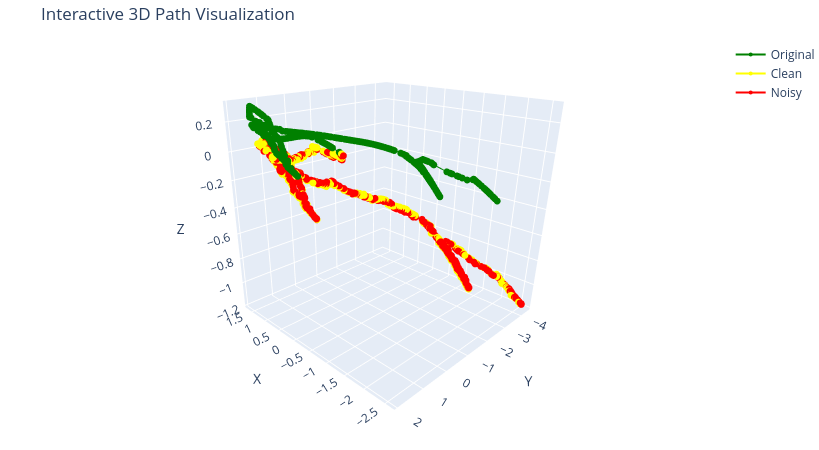
\includegraphics[width=0.7\textwidth]{full_path.png}
  \caption{Inspección visual de la trayectoria.}
\end{figure} 

\subsubsection{Métricas de Evaluación de Mapeo}

En escenarios de \textit{SLAM\cite{smith1987slam}} sin cierre de bucle, además de la trayectoria, 
es fundamental evaluar la calidad del mapa reconstruido. 
Las métricas de mapeo cuantifican tanto la exactitud de los puntos estimados 
como la cobertura de la escena.

\paragraph{\textit{Chamfer\cite{Fan2020Chamfer} Distance} (Bidireccional)}

\subparagraph{Definición matemática:}
Sea $P_{gt}$ el conjunto de puntos de referencia (ground-truth) 
y $P_{slam}$ el conjunto de puntos reconstruidos por SLAM\cite{smith1987slam}. 
La \textit{Chamfer\cite{Fan2020Chamfer} distance} bidireccional se define como:
\[
d_{CD}(P_{gt}, P_{slam}) = \frac{1}{|P_{gt}|} \sum_{p \in P_{gt}} 
\min_{q \in P_{slam}} \|p - q\|^2
+
\frac{1}{|P_{slam}|} \sum_{q \in P_{slam}} 
\min_{p \in P_{gt}} \|q - p\|^2
\]
\subparagraph{Descripción:}
Esta métrica calcula, para cada punto de un conjunto, la distancia al punto más cercano del otro conjunto y 
hace la media. La primera suma evalúa la cobertura de la reconstrucción (si faltan regiones), mientras que la 
segunda suma evalúa la exactitud (si se agregaron puntos espurios).

\paragraph{Relevancia en SLAM\cite{smith1987slam} sin cierre de bucle}
En ausencia de cierre de bucle, los mapas pueden sufrir deformaciones locales y acumulación de errores. 
La \textit{Chamfer\cite{Fan2020Chamfer} distance} permite cuantificar estas desviaciones sin requerir correspondencias explícitas de topología.

\subparagraph{Área de interés:}
\begin{itemize}
  \item Precisión global del mapa.
  \item Cobertura y completitud de la escena.
  \item Detección de artefactos o puntos espurios.
\end{itemize}

\subparagraph{Interpretación:}
\begin{itemize}
  \item Valores bajos: la reconstrucción es precisa y completa.  
  \item Valores altos en $P_{gt} \to P_{slam}$: la reconstrucción es incompleta.
  \item Valores altos en $P_{slam} \to P_{gt}$: hay puntos espurios o ruido.
\end{itemize}

\subparagraph{Resultados:}
\begin{itemize}
  \item \textbf{Ejecición sin ruido:} Los valores obtenidos son:
  \begin{itemize}
    \item \textbf{Media Original->Calculado:} 0.273 metros.
    \item \textbf{Media Calculado->Original:} 0.216 metros.
    \item \textbf{Media Chamfer\cite{Fan2020Chamfer} bidireccional:} 0.122 metros.
    \begin{figure}[h]
      \centering
        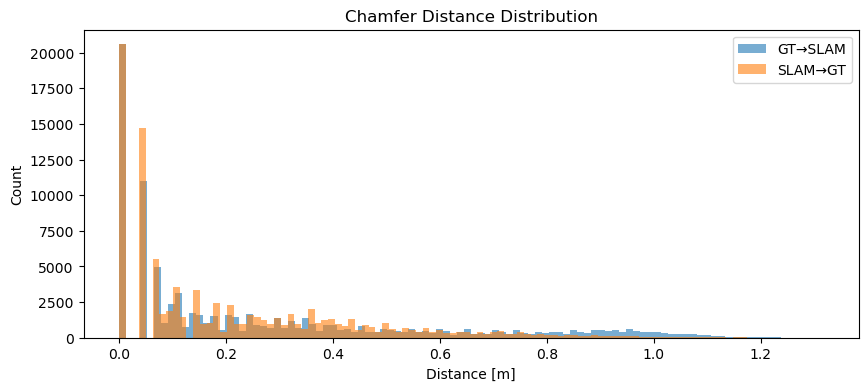
\includegraphics[width=0.5\textwidth]{chamfer_clean.png}
        \caption{Distribución de distancia entre puntos.}
    \end{figure} 
    \end{itemize}
  \newpage
  \item \textbf{Ejecición con ruido:} Los valores obtenidos son:
  \begin{itemize}
    \item \textbf{Media Original->Calculado:} 0.274 metros.
    \item \textbf{Media Calculado->Original:} 0.209 metros.
    \item \textbf{Media Chamfer\cite{Fan2020Chamfer} bidireccional:} 0.122 metros.
    \begin{figure}[h]
      \centering
        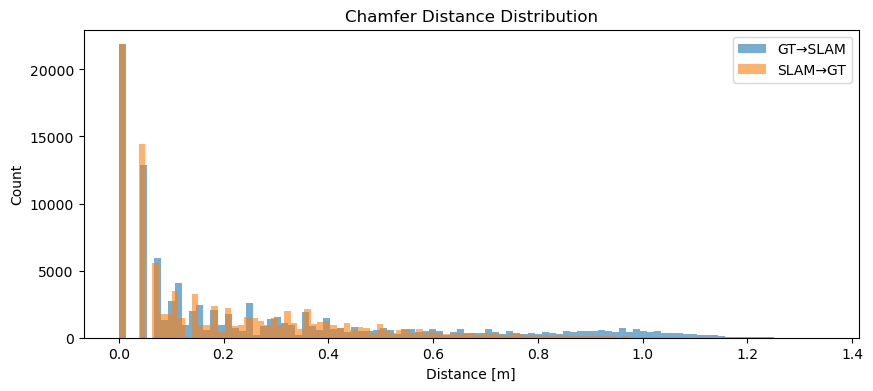
\includegraphics[width=0.5\textwidth]{chamfer_noisy.png}
      \caption{Distribución de distancia entre puntos.}
    \end{figure} 
  \end{itemize}
\end{itemize}

\subparagraph{Interpretación de resultados:}
Los resultados de la \textit{Chamfer\cite{Fan2020Chamfer} distance} bidireccional indican que el sistema de localización y mapeo logra una reconstrucción del entorno con una precisión y 
cobertura razonables en ambas ejecuciones (con y sin ruido).
En la ejecución sin ruido, la media de la distancia desde los puntos de referencia al conjunto reconstruido es de 0,273 metros,
lo que sugiere que la mayoría de los puntos del entorno están bien representados en el mapa generado.
La media en la dirección opuesta (desde el conjunto reconstruido a los puntos de referencia) es ligeramente menor, 0,216 metros,
lo que indica que hay pocos puntos espurios en la reconstrucción.\newpage 
En la ejecución con ruido, los valores son muy similares, con una media de 0,274 metros en la dirección de referencia a reconstrucción y
0,209 metros en la dirección opuesta. Esto demuestra que el sistema es robusto frente al ruido, manteniendo una calidad de reconstrucción comparable.\newline
La media bidireccional de 0,122 metros en ambas ejecuciones indica que, en promedio, los puntos del mapa están a una distancia razonable de los puntos de referencia.


\paragraph{F-score\cite{Caccia2018FScore} \(\tau\)}

\subparagraph{Definición matemática:}
Para un umbral de distancia $\tau$, se define:
\[
\text{Precision} = \frac{|\{ q \in P_{slam} : \exists p \in P_{gt}, \|q-p\| < \tau \}|}{|P_{slam}|}
\]
\[
\text{Sensibilidad} = \frac{|\{ p \in P_{gt} : \exists q \in P_{slam}, \|p-q\| < \tau \}|}{|P_{gt}|}
\]
\[
F\text{-score} = 2 \cdot \frac{\text{Precision} \cdot \text{Sensibilidad}}{\text{Precision} + \text{Sensibilidad}}
\]

\subparagraph{Descripción:}
El F-score\cite{Caccia2018FScore} combina precisión (proporción de las predicciones positivas que fueron realmente correctas) y sensibilidad (proporción de los positivos reales que fueron detectados correctamente), 
para dar un valor global de la calidad del mapa bajo un umbral de tolerancia. Si la precisión es alta pero la sensibilidad es baja, significa que la reconstrucción es precisa pero incompleta.
Si la sensibilidad es alta pero la precisión es baja, significa que la reconstrucción cubre bien la escena pero incluye muchos puntos espurios.
Se centra en si los puntos estimados están suficientemente cerca de la referencia y si la reconstrucción cubre la escena.
Esta métrica es importante en el SLAM\cite{smith1987slam} sin cierre de bucle ya que permite evaluar la calidad de la reconstrucción sin depender de la alineación 
perfecta global, lo cual es útil cuando la trayectoria ha acumulado deriva.
\subparagraph{Área de interés:}
\begin{itemize}
  \item Completitud frente a exactitud bajo un umbral de tolerancia.
  \item Comparación rápida entre distintas reconstrucciones.
  \item Evaluación de regiones críticas de la escena.
\end{itemize}

\subparagraph{Interpretación:}
\begin{itemize}
  \item F-score\cite{Caccia2018FScore} cercano a 1: buena precisión y cobertura.  
  \item Baja precisión: muchos puntos espurios.
  \item Baja sensibilidad: la reconstrucción no cubre todo el mapa.
\end{itemize}

\subparagraph{Resultados:}
\begin{itemize}
  \item \textbf{Ejecición sin ruido:} Los valores obtenidos son:
  \begin{itemize}
    \item \textbf{F-score\cite{Caccia2018FScore} \(\tau\) = 0.2 metros:} Precisión: 0.567 | Sensibilidad: 0.592 | F-score\cite{Caccia2018FScore}: 0.579.
    \item \textbf{F-score\cite{Caccia2018FScore} \(\tau\) = 0.1 metros:} Precisión: 0.428 | Sensibilidad: 0.447 | F-score\cite{Caccia2018FScore}: 0.438.
    \item \textbf{F-score\cite{Caccia2018FScore} \(\tau\) = 0.05 metros:} Precisión: 0.323 | Sensibilidad: 0.328 | F-score\cite{Caccia2018FScore}: 0.325.
  \end{itemize}
  \item \textbf{Ejecición con ruido:} Los valores obtenidos son:
  \begin{itemize}
    \item \textbf{F-score\cite{Caccia2018FScore} \(\tau\) = 0.2 metros:} Precisión: 0.573 | Sensibilidad: 0.601 | F-score\cite{Caccia2018FScore}: 0.586.
    \item \textbf{F-score\cite{Caccia2018FScore} \(\tau\) = 0.1 metros:} Precisión: 0.427 | Sensibilidad: 0.459 | F-score\cite{Caccia2018FScore}: 0.442.
    \item \textbf{F-score\cite{Caccia2018FScore} \(\tau\) = 0.05 metros:} Precisión: 0.314 | Sensibilidad: 0.338 | F-score\cite{Caccia2018FScore}: 0.325.
  \end{itemize}
\end{itemize}
\subparagraph{Interpretación de resultados:}
Los resultados del F-score\cite{Caccia2018FScore} para ambas ejecuciones (con y sin ruido) indican que el sistema de localización y mapeo logra un equilibrio razonable entre precisión y sensibilidad en la reconstrucción
del entorno.\newline
En la ejecución sin ruido, el F-score\cite{Caccia2018FScore} a un umbral de 0.2 metros es de 0.579, con una precisión del 56.7\% y una sensibilidad del 59.2\%. Esto sugiere que la mayoría de los puntos reconstruidos están
cerca de los puntos de referencia y que la reconstrucción cubre una parte significativa de la escena.
A medida que se reduce el umbral a 0.1 y 0.05 metros, el F-score\cite{Caccia2018FScore} disminuye, lo cual es esperado, ya que es más difícil cumplir con criterios más estrictos.\newline
En la ejecución con ruido, los valores del F-score\cite{Caccia2018FScore} son ligeramente mejores, con un F-score\cite{Caccia2018FScore} de 0.586 a un umbral de 0.2 metros. La precisión y sensibilidad también son marginalmente superiores en 
comparación con la ejecución sin ruido.
Esto podría indicar que el sistema es capaz de manejar el ruido de manera efectiva, manteniendo una calidad de reconstrucción comparable.\newline
En general, los resultados sugieren que el sistema de localización y mapeo es robusto y capaz de producir mapas de calidad razonable, incluso en presencia de ruido.

\paragraph{Distribución de Errores (Percentiles)}

\subparagraph{Definición matemática:}
Sea $d_i = \min_{q \in P_{slam}} \|p_i - q\|$ la distancia del punto $p_i \in P_{gt}$ a su vecino más cercano en $P_{slam}$.  
Se calculan percentiles $p_{50}, p_{90}, p_{95}, p_{99}$ del conjunto $\{d_i\}$:
\[
p_x = \text{percentil}_x(\{ d_i \})
\]

\subparagraph{Descripción:}
consiste en analizar cómo se distribuyen las diferencias entre el mapa generado y el mapa de referencia, expresadas como error por vóxel.
 En lugar de usar solo un promedio, se calculan percentiles (p. ej., 25, 50, 75, 95) para identificar la variabilidad del error en todo el 
 volumen. Esto permite detectar si los errores se concentran en pocas regiones (colas de la distribución) o si están repartidos de forma 
 uniforme, proporcionando una visión más robusta y detallada de la calidad del modelo.

\subparagraph{Relevancia en SLAM\cite{smith1987slam} sin cierre de bucle:}
Es especialmente útil para detectar zonas donde la reconstrucción falla debido a deriva local, ya que puede haber outliers 
importantes incluso si la mayoría de la nube es correcta.
\subparagraph{Área de interés:}
\begin{itemize}
  \item Errores típicos y extremos.
  \item Detección de outliers.
  \item Evaluación de robustez local de la reconstrucción.
\end{itemize}

\subparagraph{Interpretación:}
\begin{itemize}
  \item $p_{50}$: error típico de la mayoría de puntos.  
  \item $p_{90}$, $p_{95}$: errores significativos de regiones concretas.  
  \item $p_{99}$: outliers extremos.  
  \item Los histogramas de error ayudan a identificar patrones de error espacial.
\end{itemize}

\subparagraph{Resultados:}
\begin{itemize}
  \item \textbf{Ejecución sin ruido:} Los valores obtenidos son:
  \begin{itemize}
    \item \textbf{Mediana:} 0.141 metros. 
    \item \textbf{P90:} 0.825 metros.
    \item \textbf{P95:} 0.953 metros.
    \item \textbf{P99:} 1.083 metros.
    \begin{figure}[h]
      \centering
        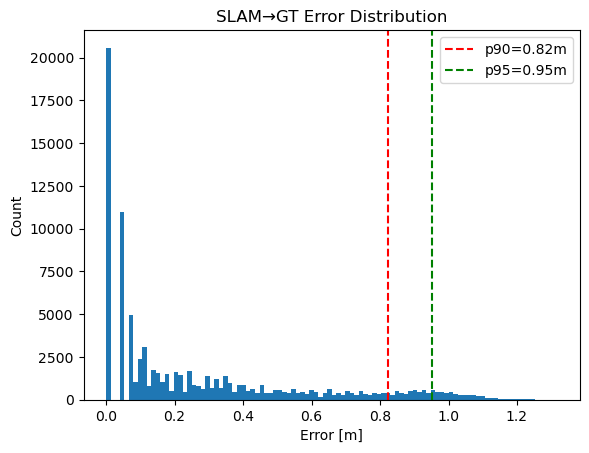
\includegraphics[width=0.5\textwidth]{ed_clean.png}
        \caption{Distribución de distancia entre puntos.}
    \end{figure} 
    \end{itemize}
  \item \textbf{Ejecución con ruido:} Los valores obtenidos son:
  \begin{itemize}
    \item \textbf{Mediana:} 0.141 metros. 
    \item \textbf{P90:} 0.844 metros.
    \item \textbf{P95:} 0.976 metros.
    \item \textbf{P99:} 1.108 metros.
    \begin{figure}[h]
      \centering
        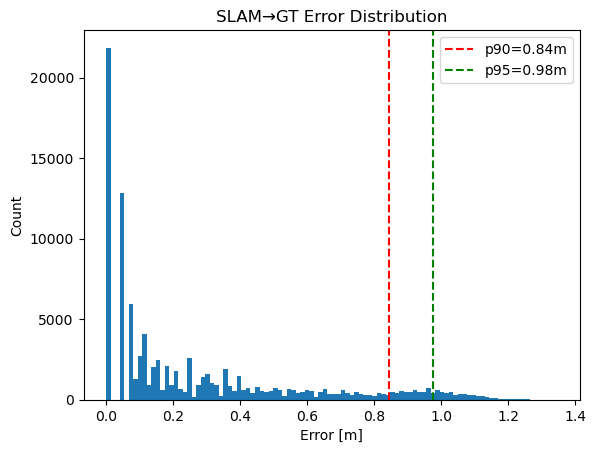
\includegraphics[width=0.5\textwidth]{ed_noisy.png}
      \caption{Distribución de distancia entre puntos.}
    \end{figure} 
  \end{itemize}
\end{itemize}
\subparagraph{Interpretación de resultados:}
Los resultados de la distribución de errores para ambas ejecuciones (con y sin ruido) indican que el sistema de localización y mapeo logra una reconstrucción del entorno con una precisión razonable.
En la ejecución sin ruido, la mediana del error es de 0.141 metros, lo que sugiere que la mayoría de los puntos del entorno están bien representados en el mapa generado.
El percentil 90 (P90) es de 0.825 metros, lo que indica que el 90\% de los puntos tienen un error menor a este valor.
Los percentiles 95 (P95) y 99 (P99) son de 0.953 metros y 1.083 metros, respectivamente, lo que sugiere que hay algunos puntos con errores más significativos, pero estos son relativamente pocos.
En la ejecución con ruido, los valores son muy similares, con una mediana del error también de 0.141 metros.
El P90 aumenta ligeramente a 0.844 metros, y los P95 y P99 también muestran un ligero incremento.
Esto demuestra que el sistema es robusto frente al ruido, manteniendo una calidad de reconstrucción comparable.
En general, los resultados sugieren que el sistema de localización y mapeo es capaz de producir mapas de calidad razonable, incluso en presencia de ruido, con la mayoría de los puntos teniendo errores moderados 
y solo unos pocos outliers con errores más grandes.

\paragraph{Resumen de métricas de mapeo}
En resumen, las métricas de mapeo (Chamfer\cite{Fan2020Chamfer} distance bidireccional, F-score\cite{Caccia2018FScore} y distribución de errores) proporcionan una visión completa del rendimiento del sistema de localización y mapeo en términos de calidad del mapa reconstruido.
La Chamfer\cite{Fan2020Chamfer} distance evalúa tanto la precisión como la cobertura del mapa, el F-score\cite{Caccia2018FScore} combina precisión y sensibilidad bajo distintos umbrales de tolerancia, y la distribución de errores ofrece una visión detallada de la variabilidad del error en todo el volumen.
Los resultados obtenidos en ambas ejecuciones (con y sin ruido) demuestran que el sistema es robusto y capaz de producir mapas de calidad razonable, incluso en presencia de ruido.
Estas métricas son fundamentales para validar la eficacia del sistema en escenarios de SLAM\cite{smith1987slam} sin cierre de bucle. Además, haciendo una inspección visual del mapa, se puede observar que el sistema logra reconstruir de manera bastante fiel la estructura del entorno,
con algunas desviaciones que se corresponden con los errores cuantificados por las métricas.

\begin{figure}[h]
  \centering
    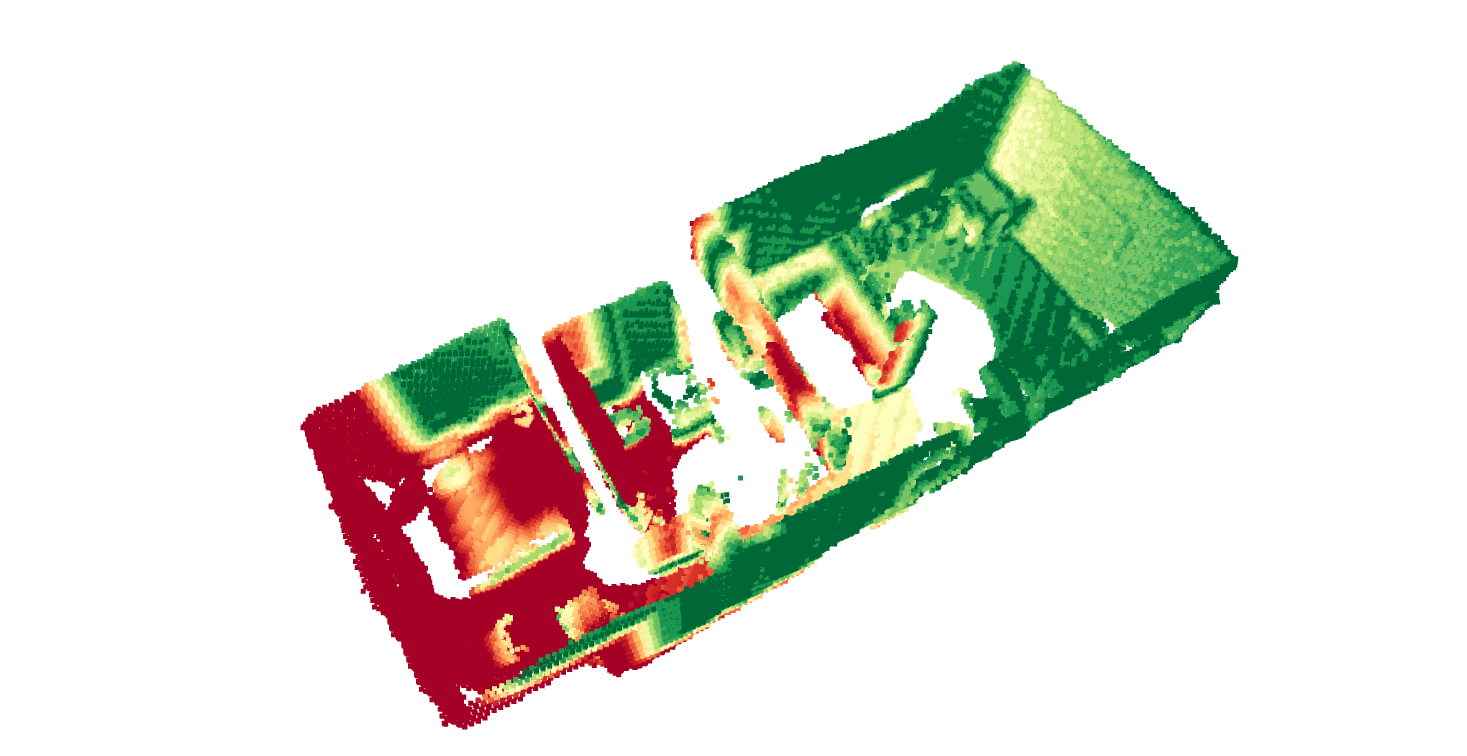
\includegraphics[width=0.5\textwidth]{map_clean.png}
  \caption{Inspección visual del mapa (ejecución sin ruido).}
\end{figure} 

\begin{figure}[h]
  \centering
    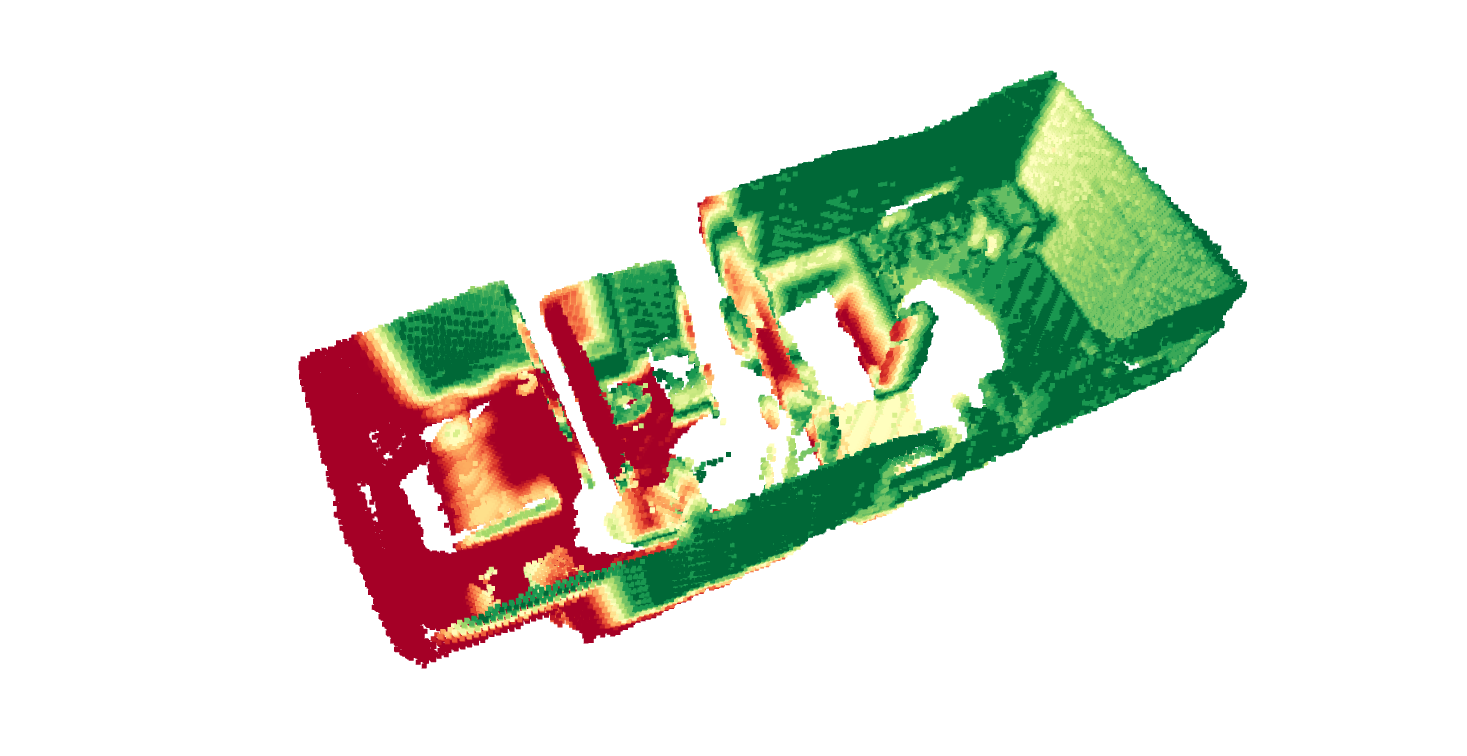
\includegraphics[width=0.5\textwidth]{map_noisy.png}
  \caption{Distribución de distancia entre puntos (con ruido).}
\end{figure} 

\section{Conclusiones y trabajo futuro}
En este proyecto se ha desarrollado un sistema de localización y mapeo basado en nubes de puntos 3D, utilizando algoritmos de ICP para la estimación de la pose y la integración de nubes de puntos en un mapa 
3D mediante la librería Bonxai. El sistema ha sido implementado en ROS2\cite{doi:10.1126/scirobotics.abm6074}, lo que facilita su integración con otros componentes robóticos y su despliegue en entornos reales.\newline
Las pruebas realizadas han demostrado que el sistema es capaz de estimar la trayectoria del robot con una precisión razonable, incluso en presencia de ruido en las nubes de puntos. Las métricas de
evaluación, como el ATE\cite{Chen2022DELOATE}, RPE\cite{Sturm2012RPE} y KITTI-style drift\cite{Geiger2013KITTI}, han mostrado resultados satisfactorios, indicando que el sistema es robusto y preciso.\newline
En cuanto a la construcción del mapa, las métricas de Chamfer\cite{Fan2020Chamfer} distance y F-score\cite{Caccia2018FScore} han confirmado que el sistema puede generar mapas 3D de calidad, con una buena cobertura y precisión en la 
representación del entorno.\newline

A pesar de los resultados positivos, existen varias áreas de mejora y trabajo futuro. En primer lugar, se podría explorar la integración de técnicas de aprendizaje automático para mejorar la robustez del
algoritmo de ICP, especialmente en entornos con alta densidad de ruido o con estructuras repetitivas. Además, la incorporación de sensores adicionales, como cámaras RGB y sensores de odometría, 
podría mejorar la precisión de la estimación de la pose y la calidad del mapa.\newline
Otra línea de trabajo futuro es la optimización del rendimiento computacional del sistema, para permitir su uso en tiempo real en robots móviles con recursos limitados. Esto podría incluir la 
implementación de versiones que usen el hardware dedicado de forma eficiente, como aceleradores para los algoritmos de ICP, y la optimización del proceso de integración de nubes de 
puntos en Bonxai\cite{faconti2024bonxai}.\newline
También sería interesante explorar la extensión del sistema para soportar el cierre de bucle, lo que permitiría corregir la deriva acumulada en la estimación de la trayectoria y mejorar la calidad del mapa
a largo plazo.\newline

En resumen, este proyecto ha sentado las bases para un sistema de localización y mapeo basado en nubes de puntos 3D, demostrando su viabilidad y eficacia. Con las mejoras propuestas, el sistema podría
ser adaptado para una amplia gama de aplicaciones robóticas, desde la navegación autónoma hasta la inspección y mapeo de entornos complejos.

\bibliographystyle{ieeetr} % Puedes usar plain, alpha, apalike, etc.
\bibliography{references}

%% Apendices
\begin{umaappendices}
\section{Código Fuente}
Todo el código desarrollado para este proyecto está disponible en el siguiente repositorio de GitHub\cite{github}: \href{https://github.com/Pablovv56/TFG.git}{https://github.com/Pablovv56/TFG.git}
\end{umaappendices}


\includepdf[noautoscale=true, width=\paperwidth]{contraportada.pdf}

\end{document}
